\documentclass[tikz, border=5mm]{standalone}
\usepackage{tikz}
\usepackage{amsmath}
\usepackage{amssymb}
\usepackage{mathtools}
\usepackage{physics}
\usetikzlibrary{arrows.meta, positioning, calc}
\begin{document}

\begin{tikzpicture}
  % Define box size and gap
  \def\boxsize{2cm}
  \def\gap{4mm}

  % Draw five boxes with gradient fill manually (gradient upwards)
  \shade[bottom color=blue!20, top color=white] (-\gap,0) rectangle ++(\boxsize, \boxsize);
  \draw[thick] (-\gap,0) rectangle ++(\boxsize, \boxsize)node (A){};
  \node[opacity=0.8] at (\boxsize/2-\gap, \boxsize/2 - 0.5em) {
    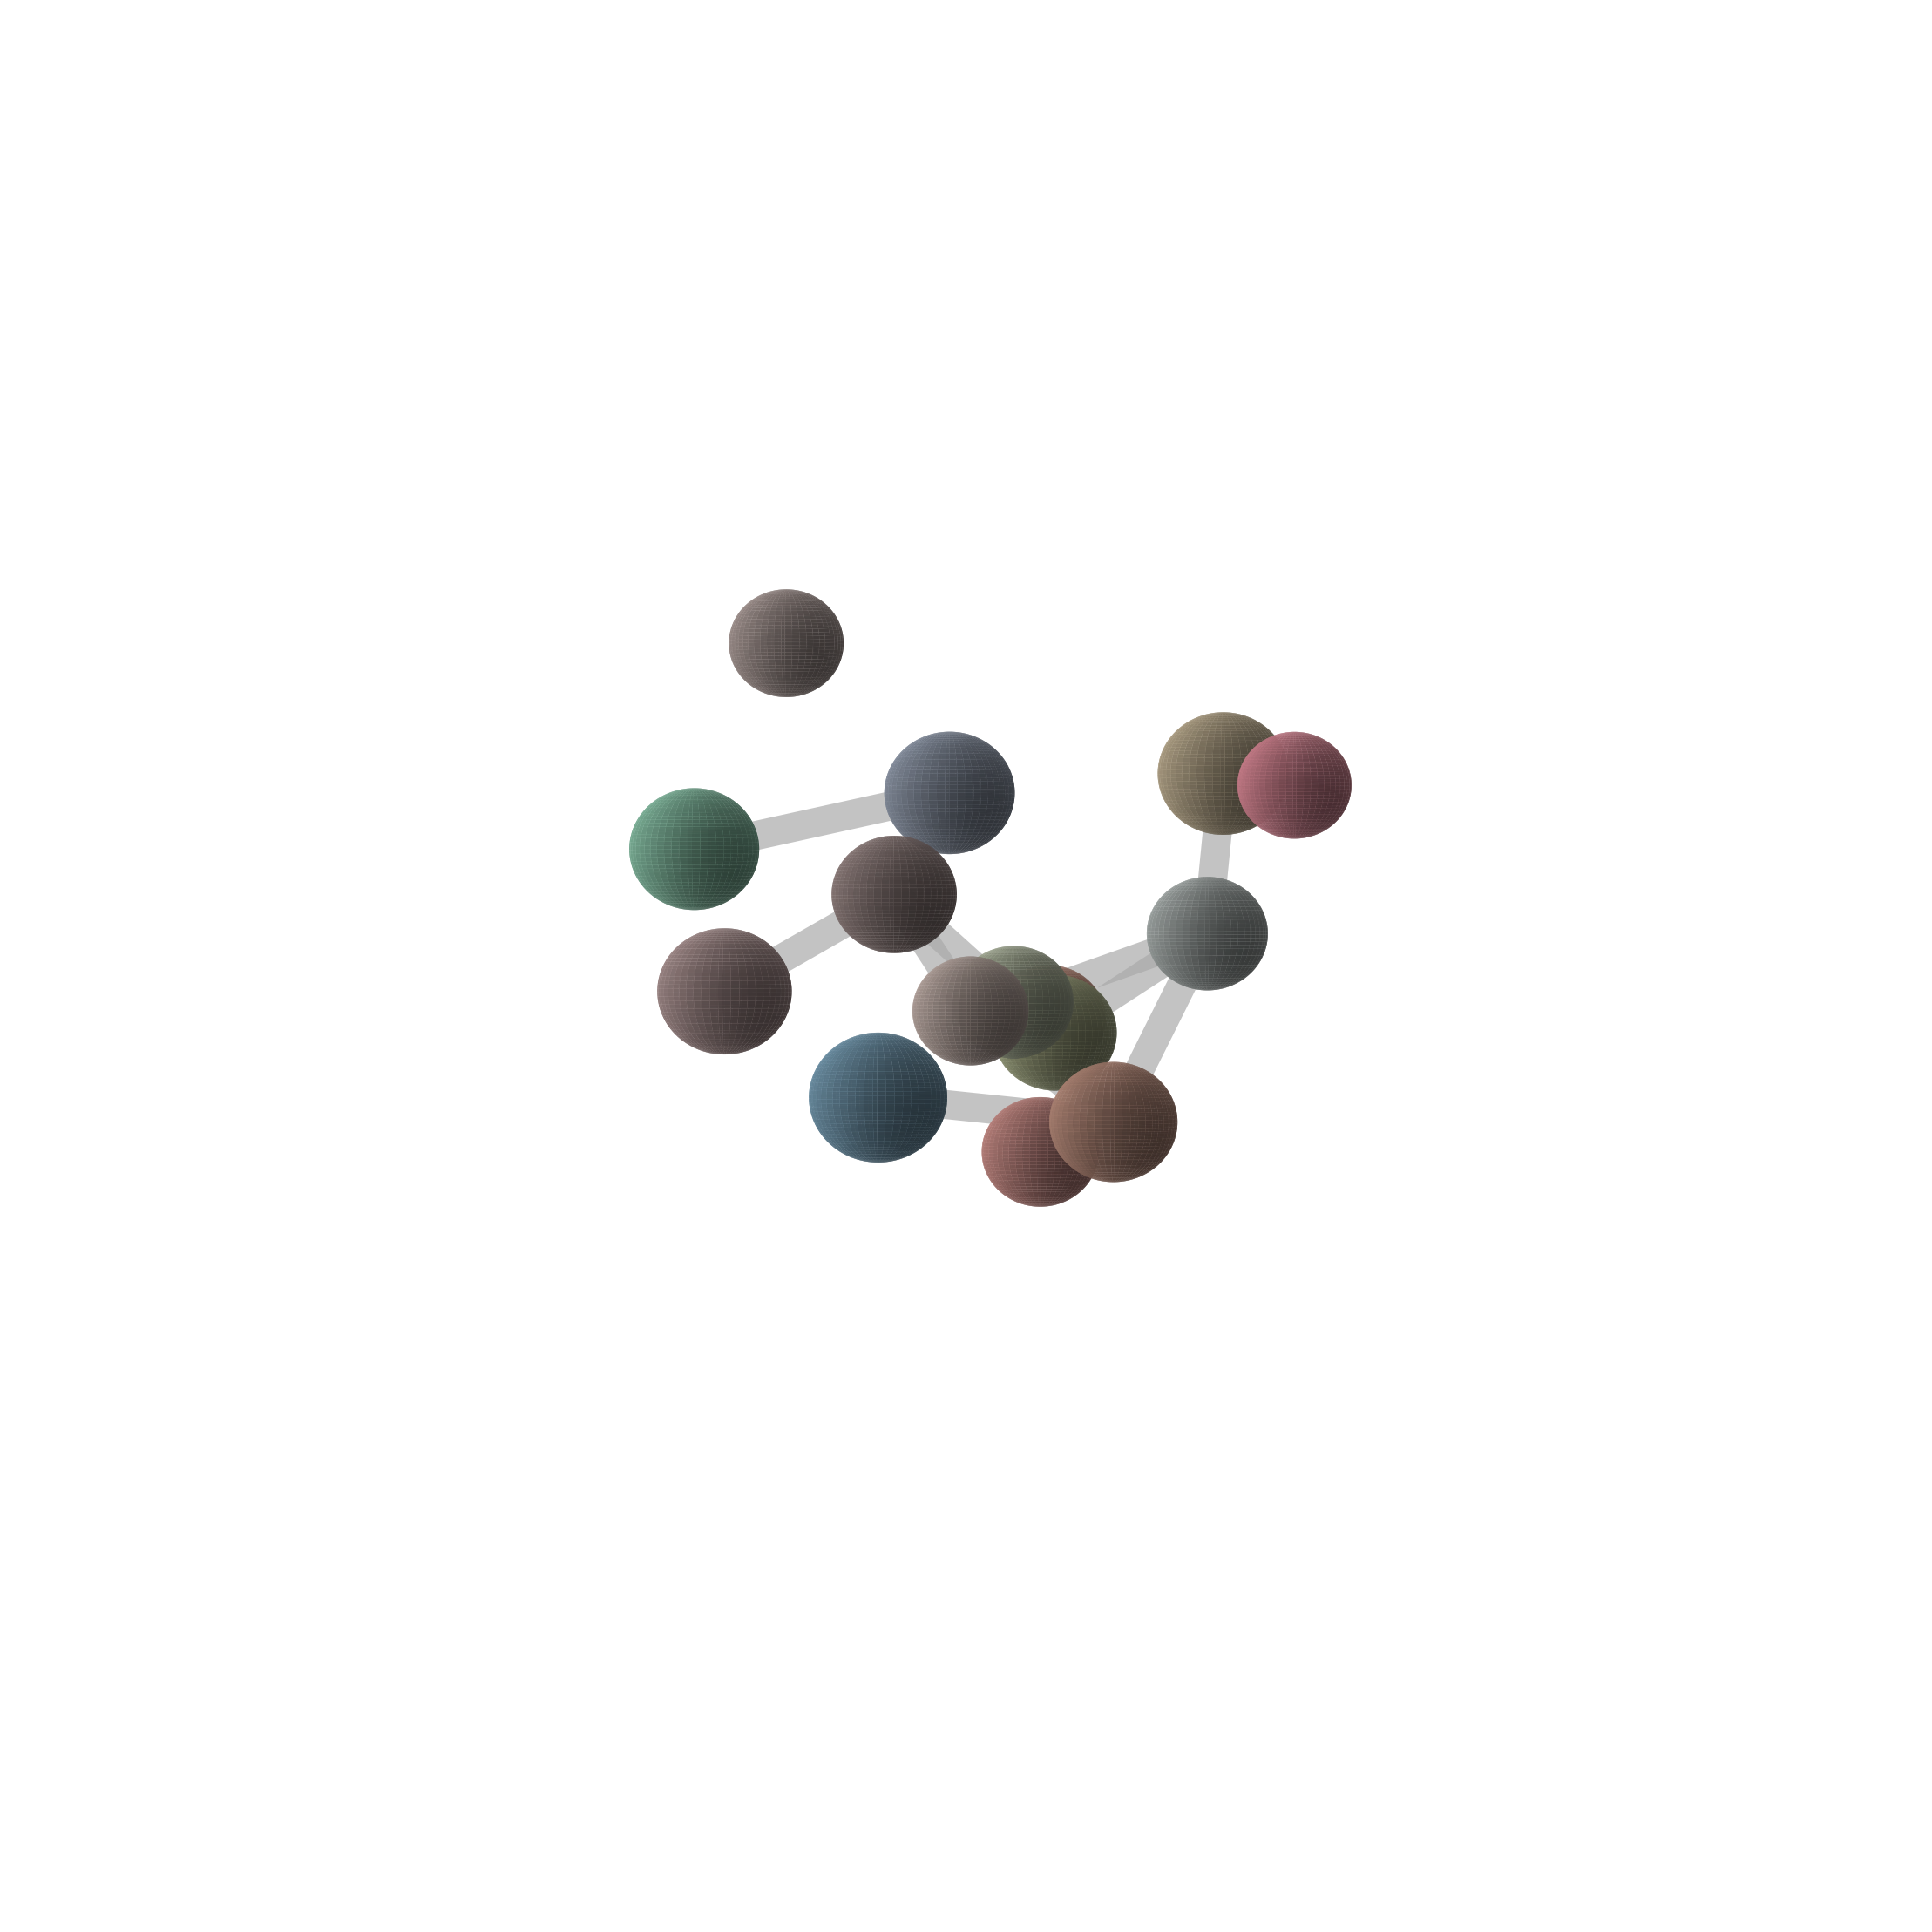
\includegraphics[width=\boxsize,height=\boxsize]{step_images/image_0.png}
  };
  \node[opacity=0.8] at (\boxsize/2-\gap, \boxsize/2 - 0.5em) {
    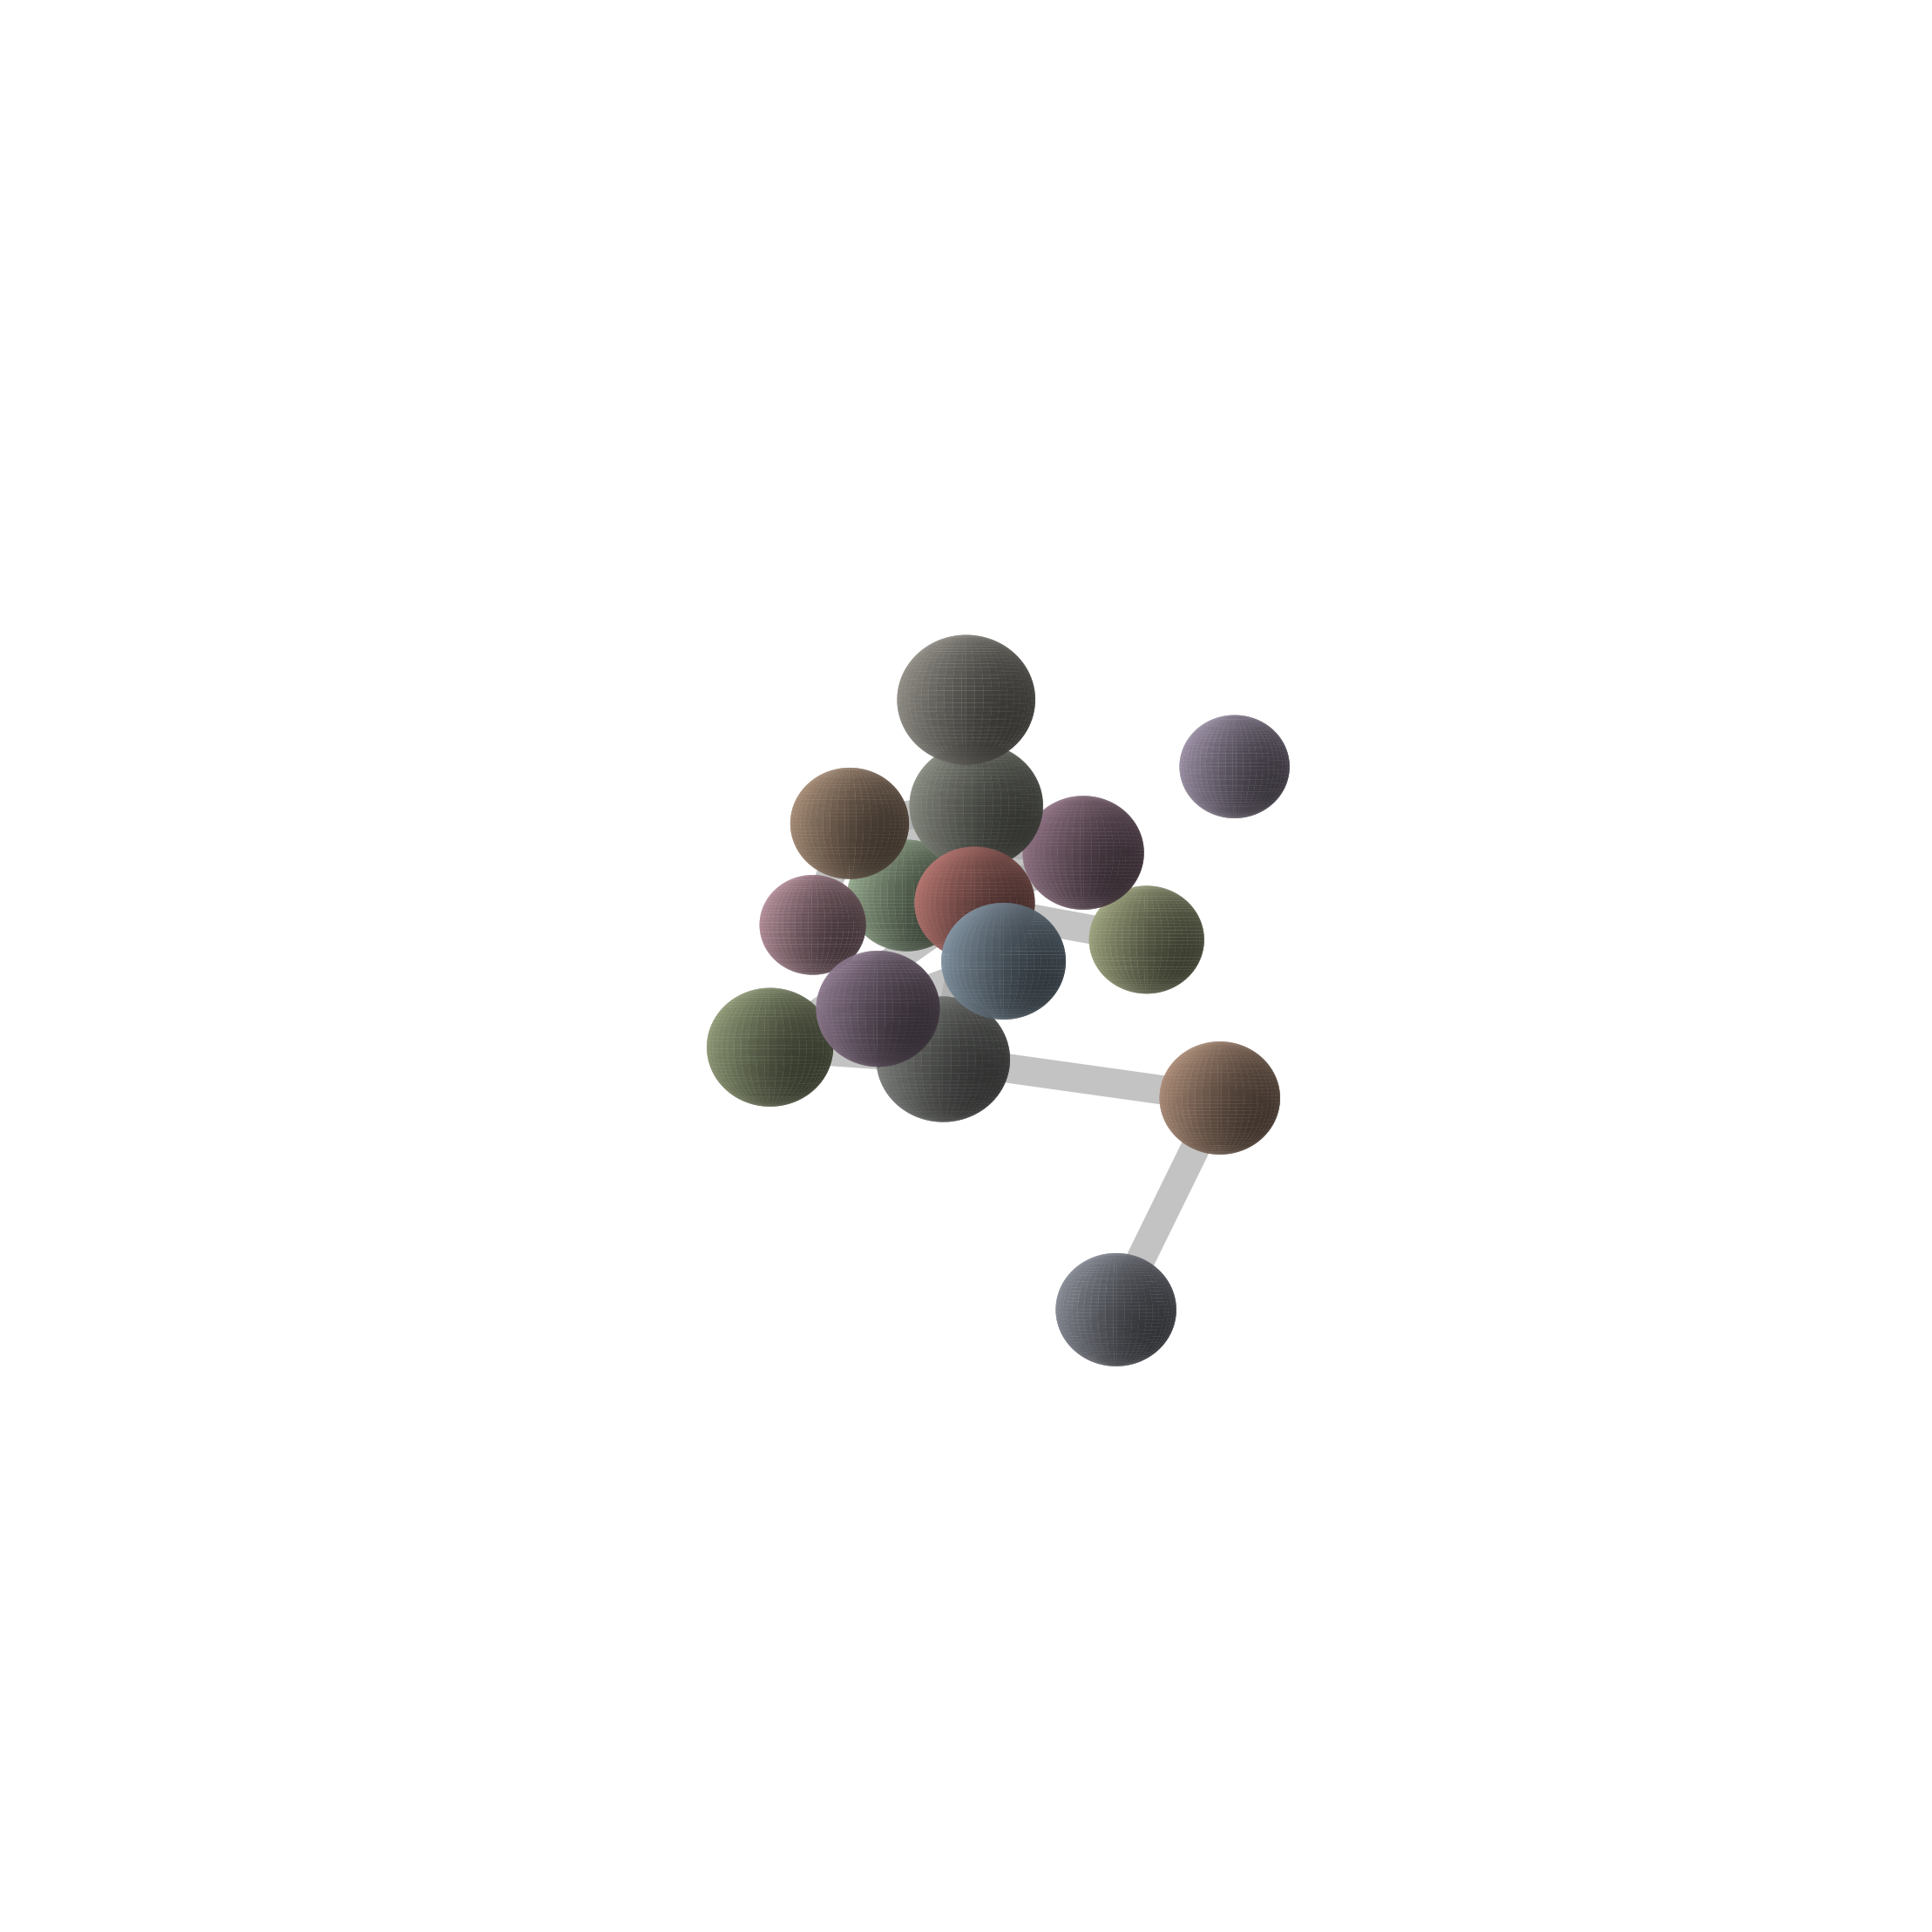
\includegraphics[width=\boxsize,height=\boxsize]{step_images/image_5.png}
  };
  \node[opacity=0.8] at (\boxsize/2-\gap, \boxsize/2 - 0.5em) {
    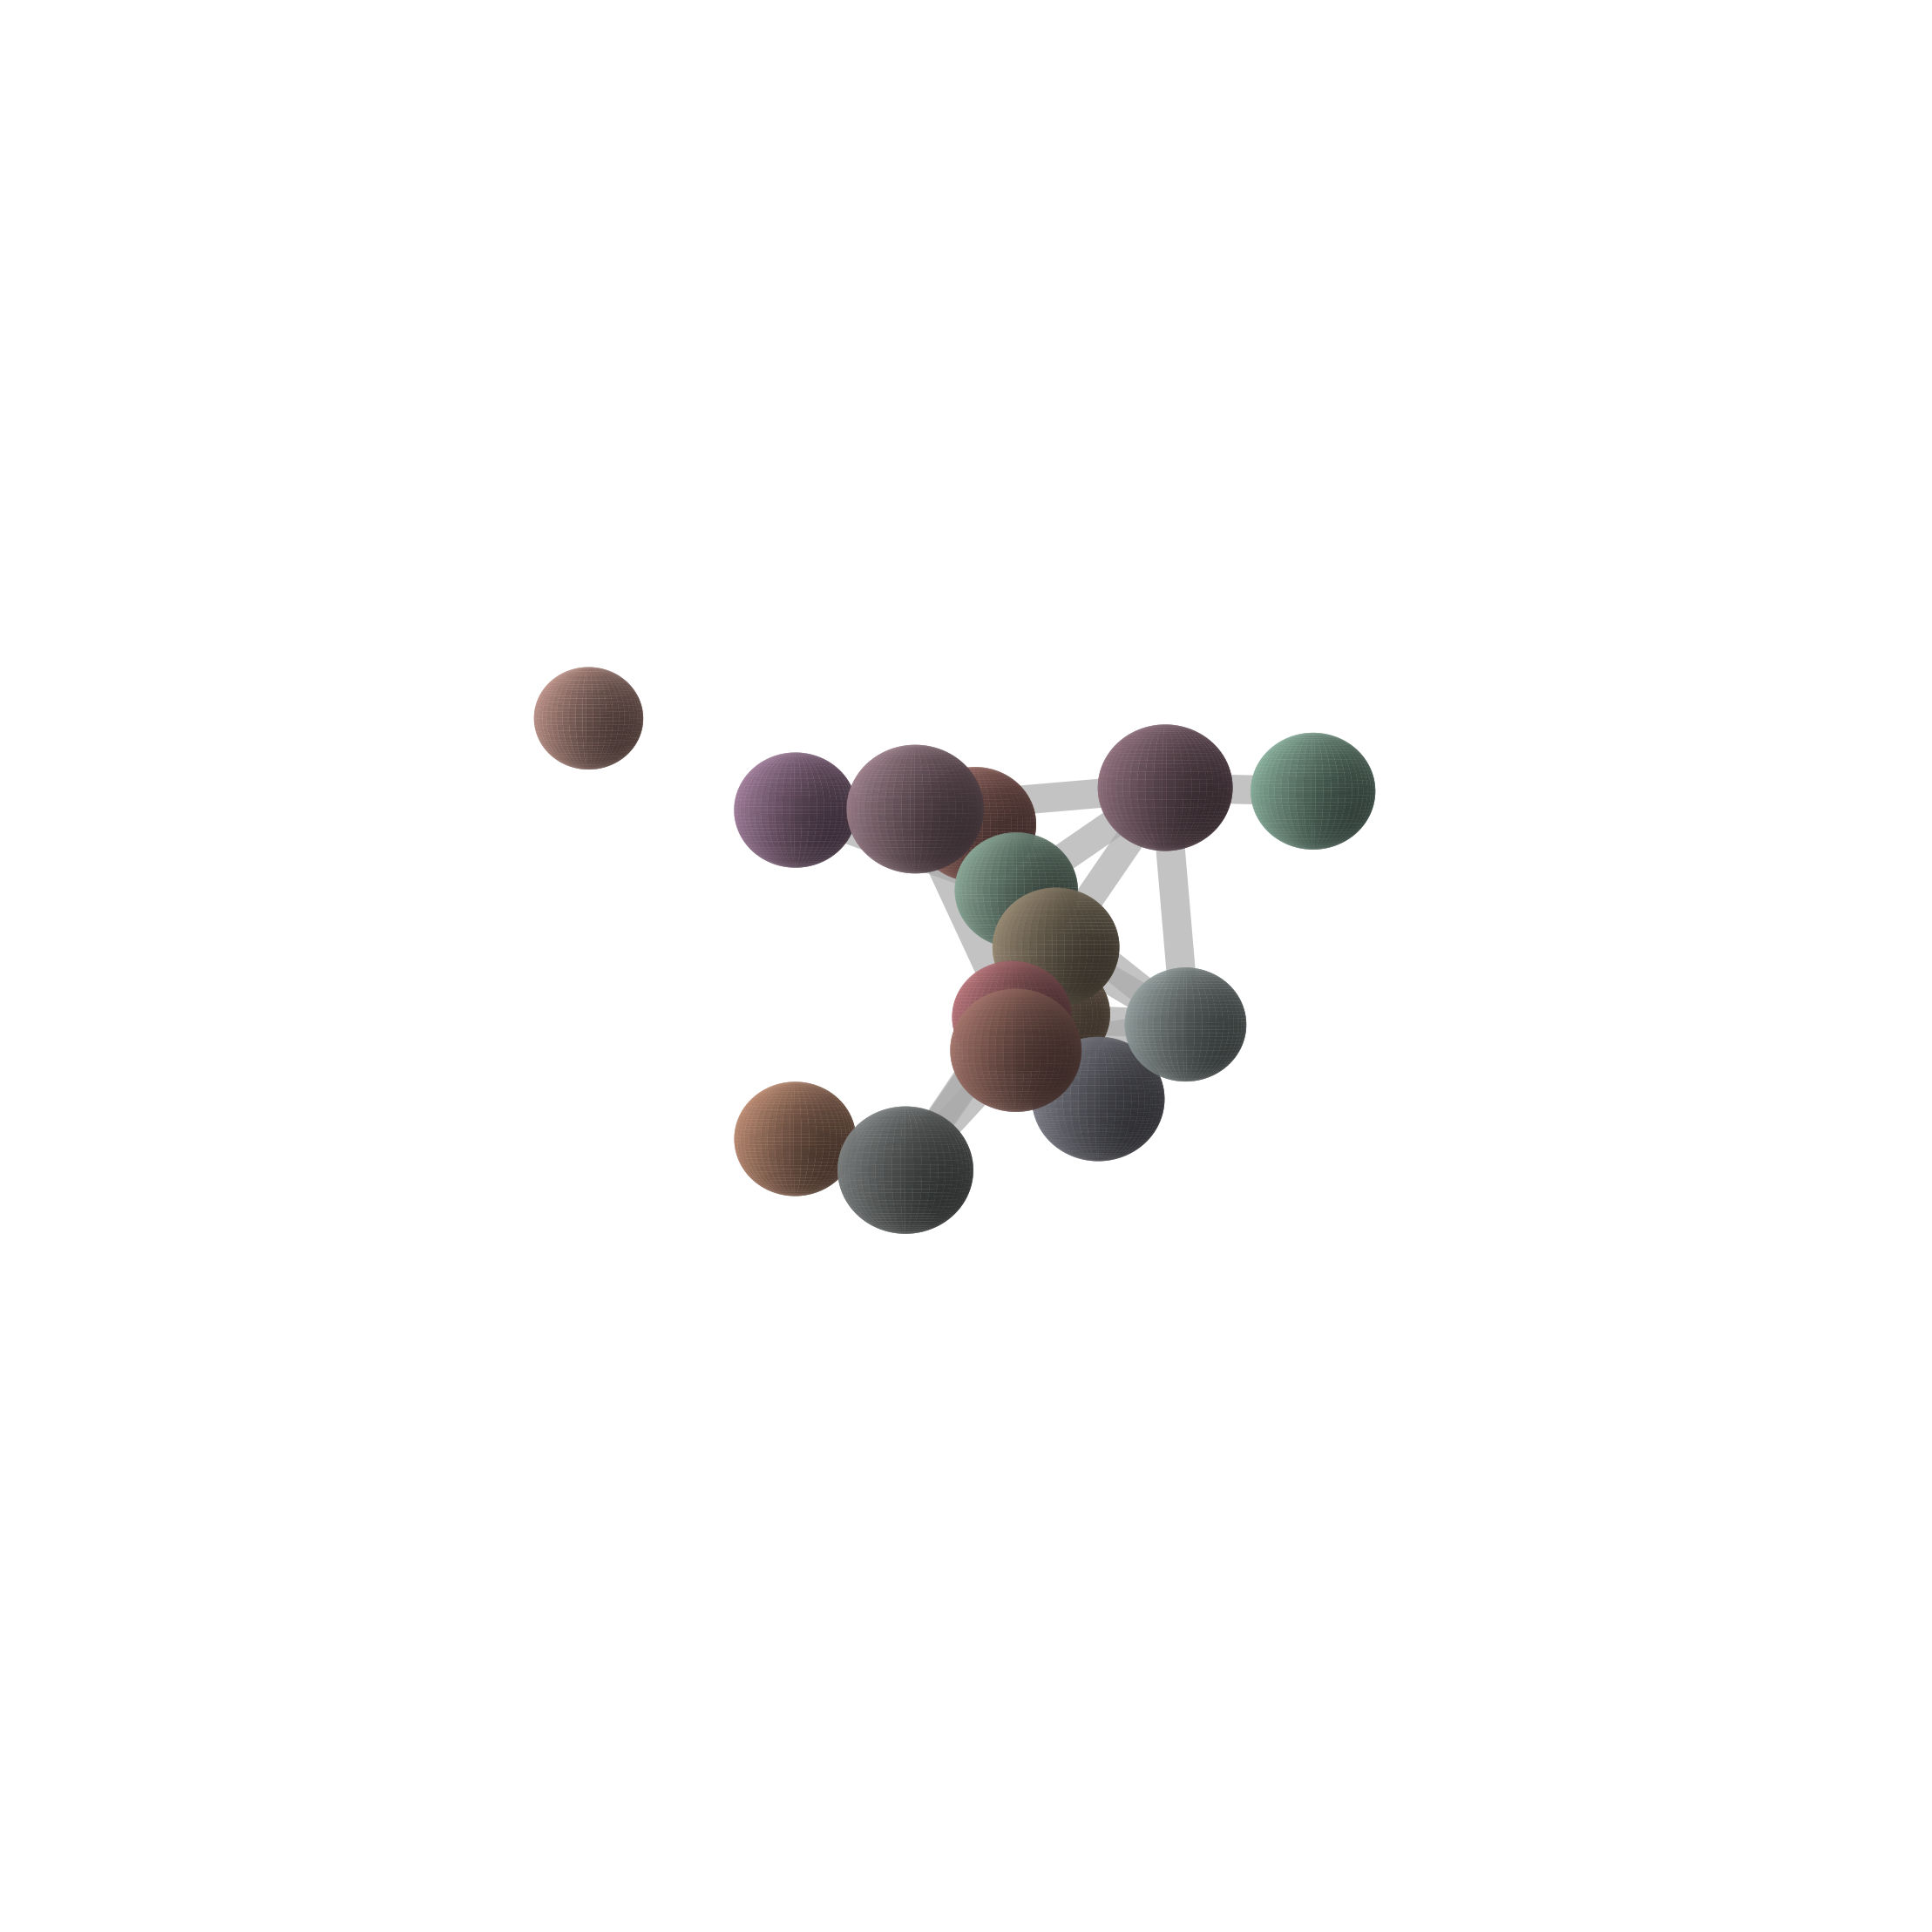
\includegraphics[width=\boxsize,height=\boxsize]{step_images/image_10.png}
  };

  \shade[bottom color=blue!20, top color=white] (\boxsize + \gap,0) rectangle ++(\boxsize, \boxsize);
  \draw[thick] (\boxsize + \gap,0) rectangle ++(\boxsize, \boxsize)node (B){};
  \node[opacity=0.8] at (1.5*\boxsize + \gap, \boxsize/2 - 0.5em) {
    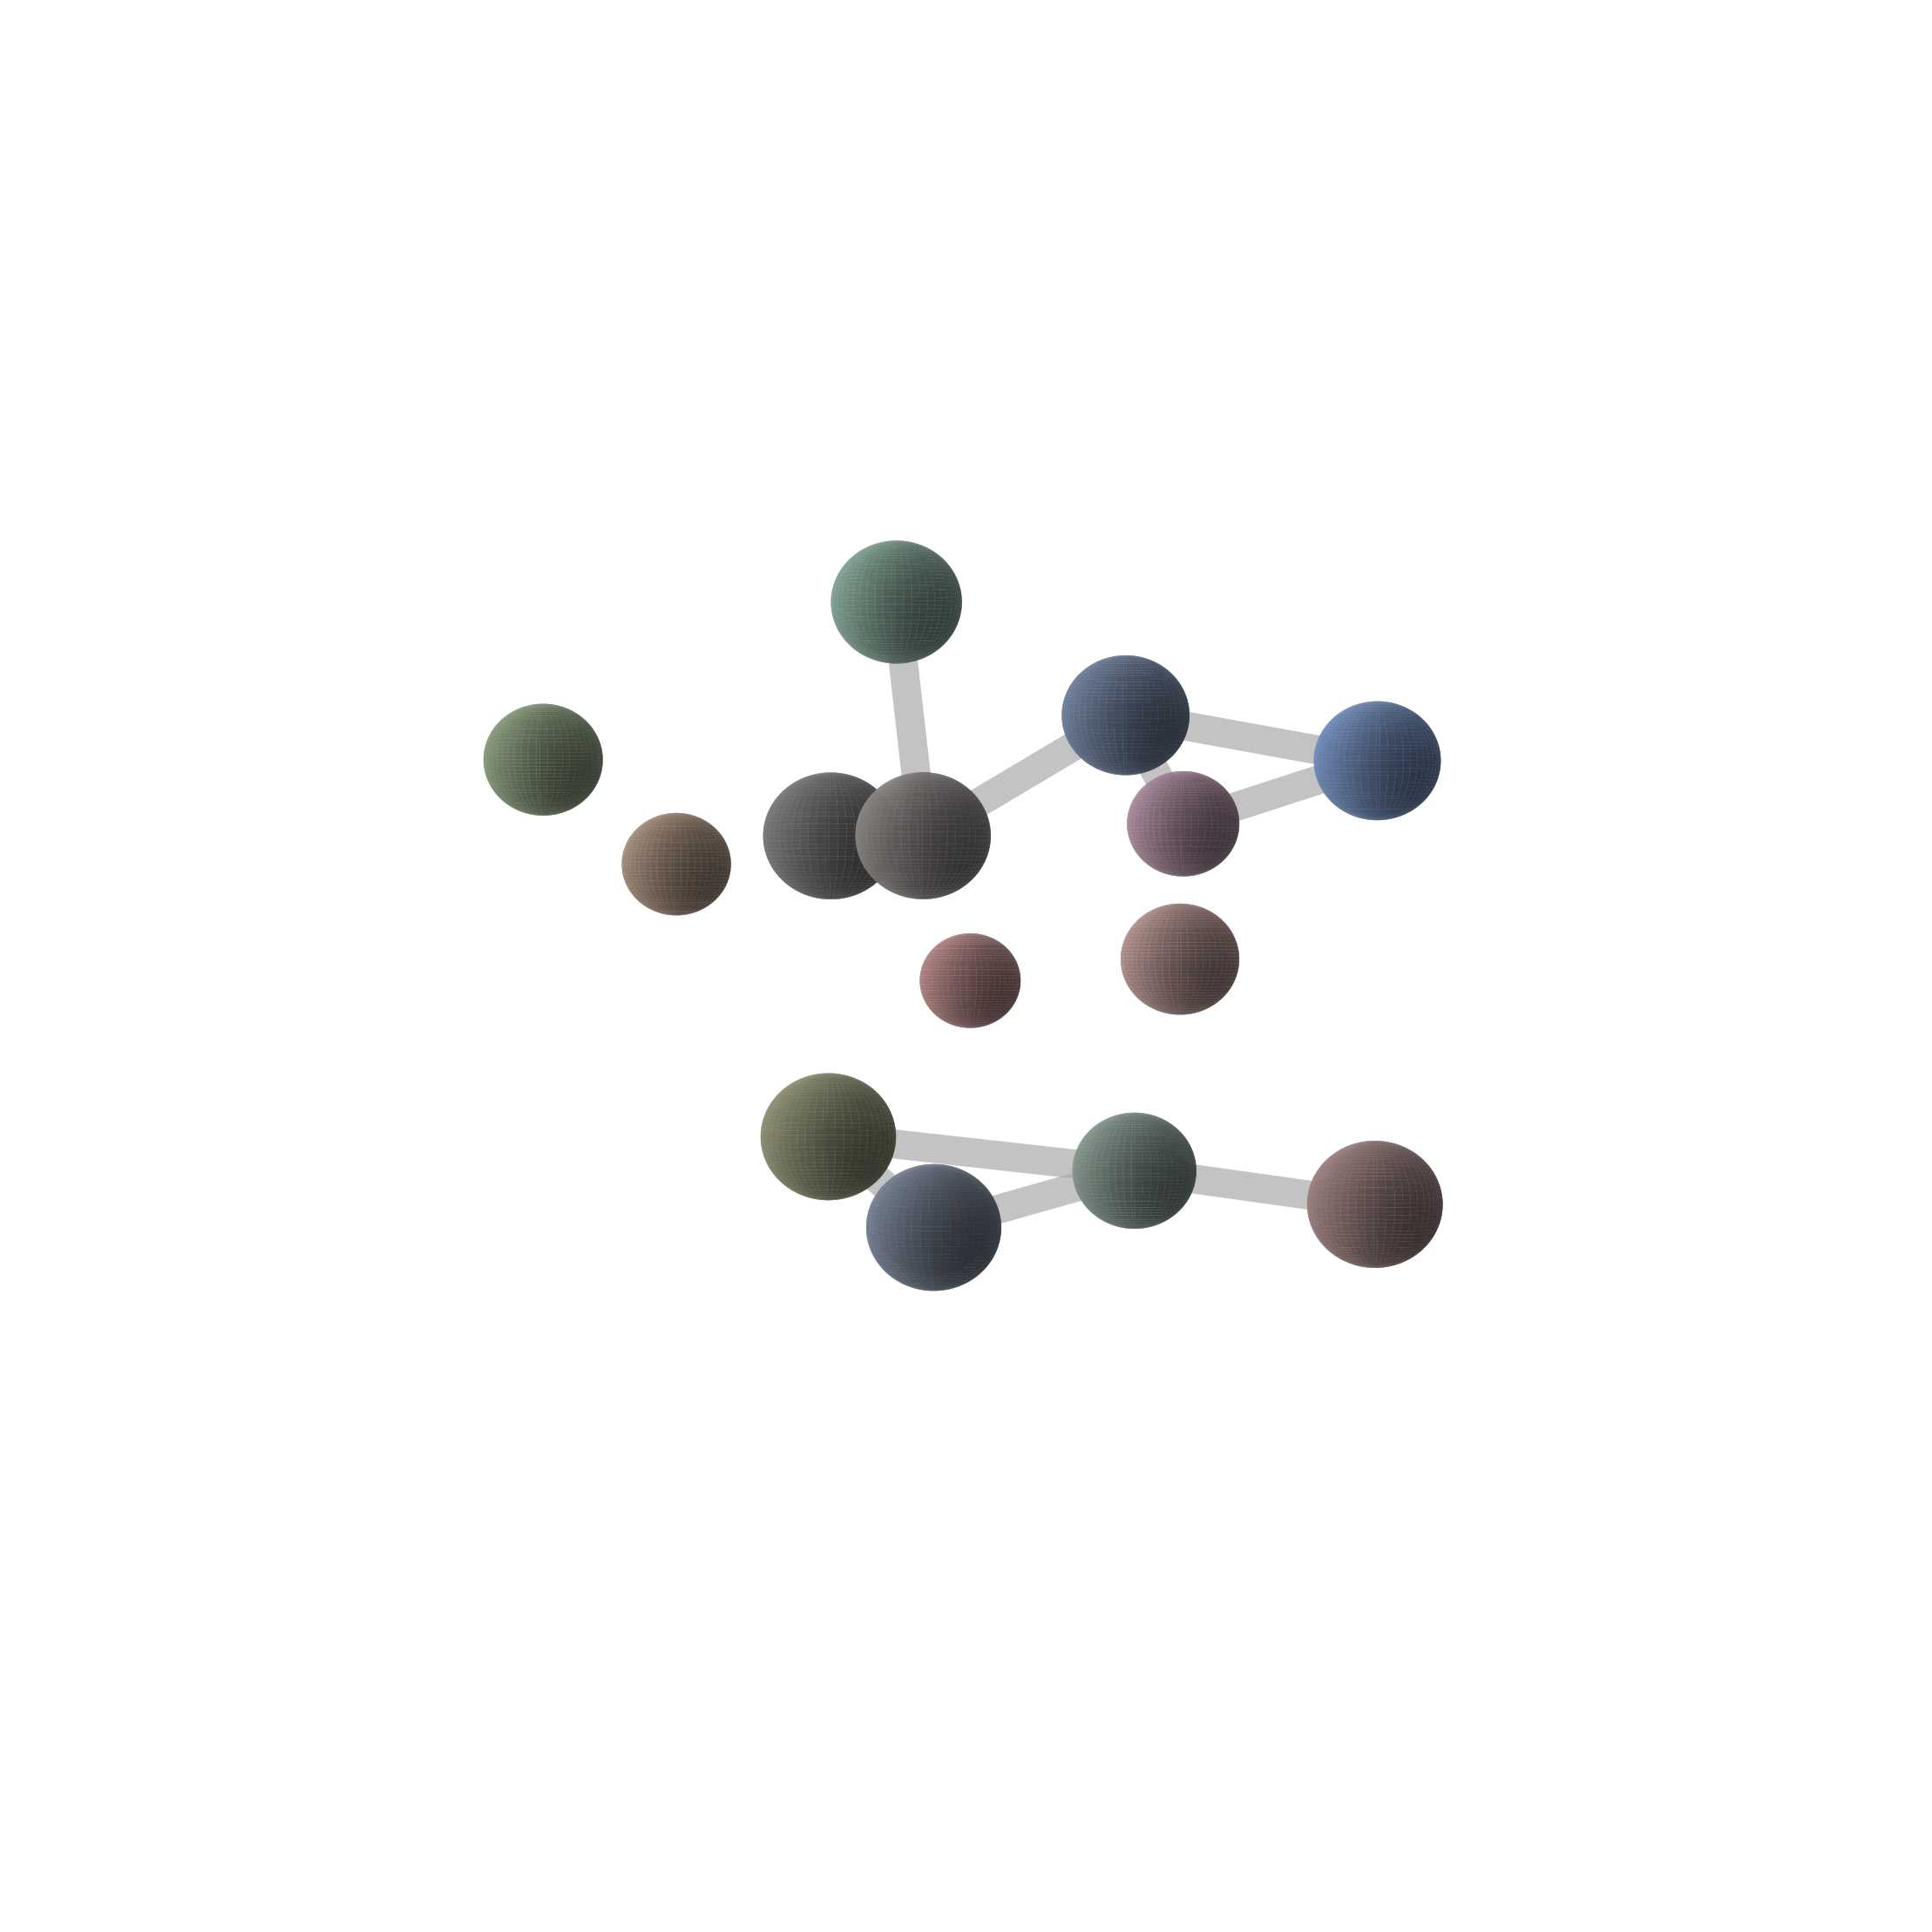
\includegraphics[width=\boxsize,height=\boxsize]{step_images/image_200.png}
  };
  \node[opacity=0.8] at (1.5*\boxsize + \gap, \boxsize/2 - 0.5em) {
    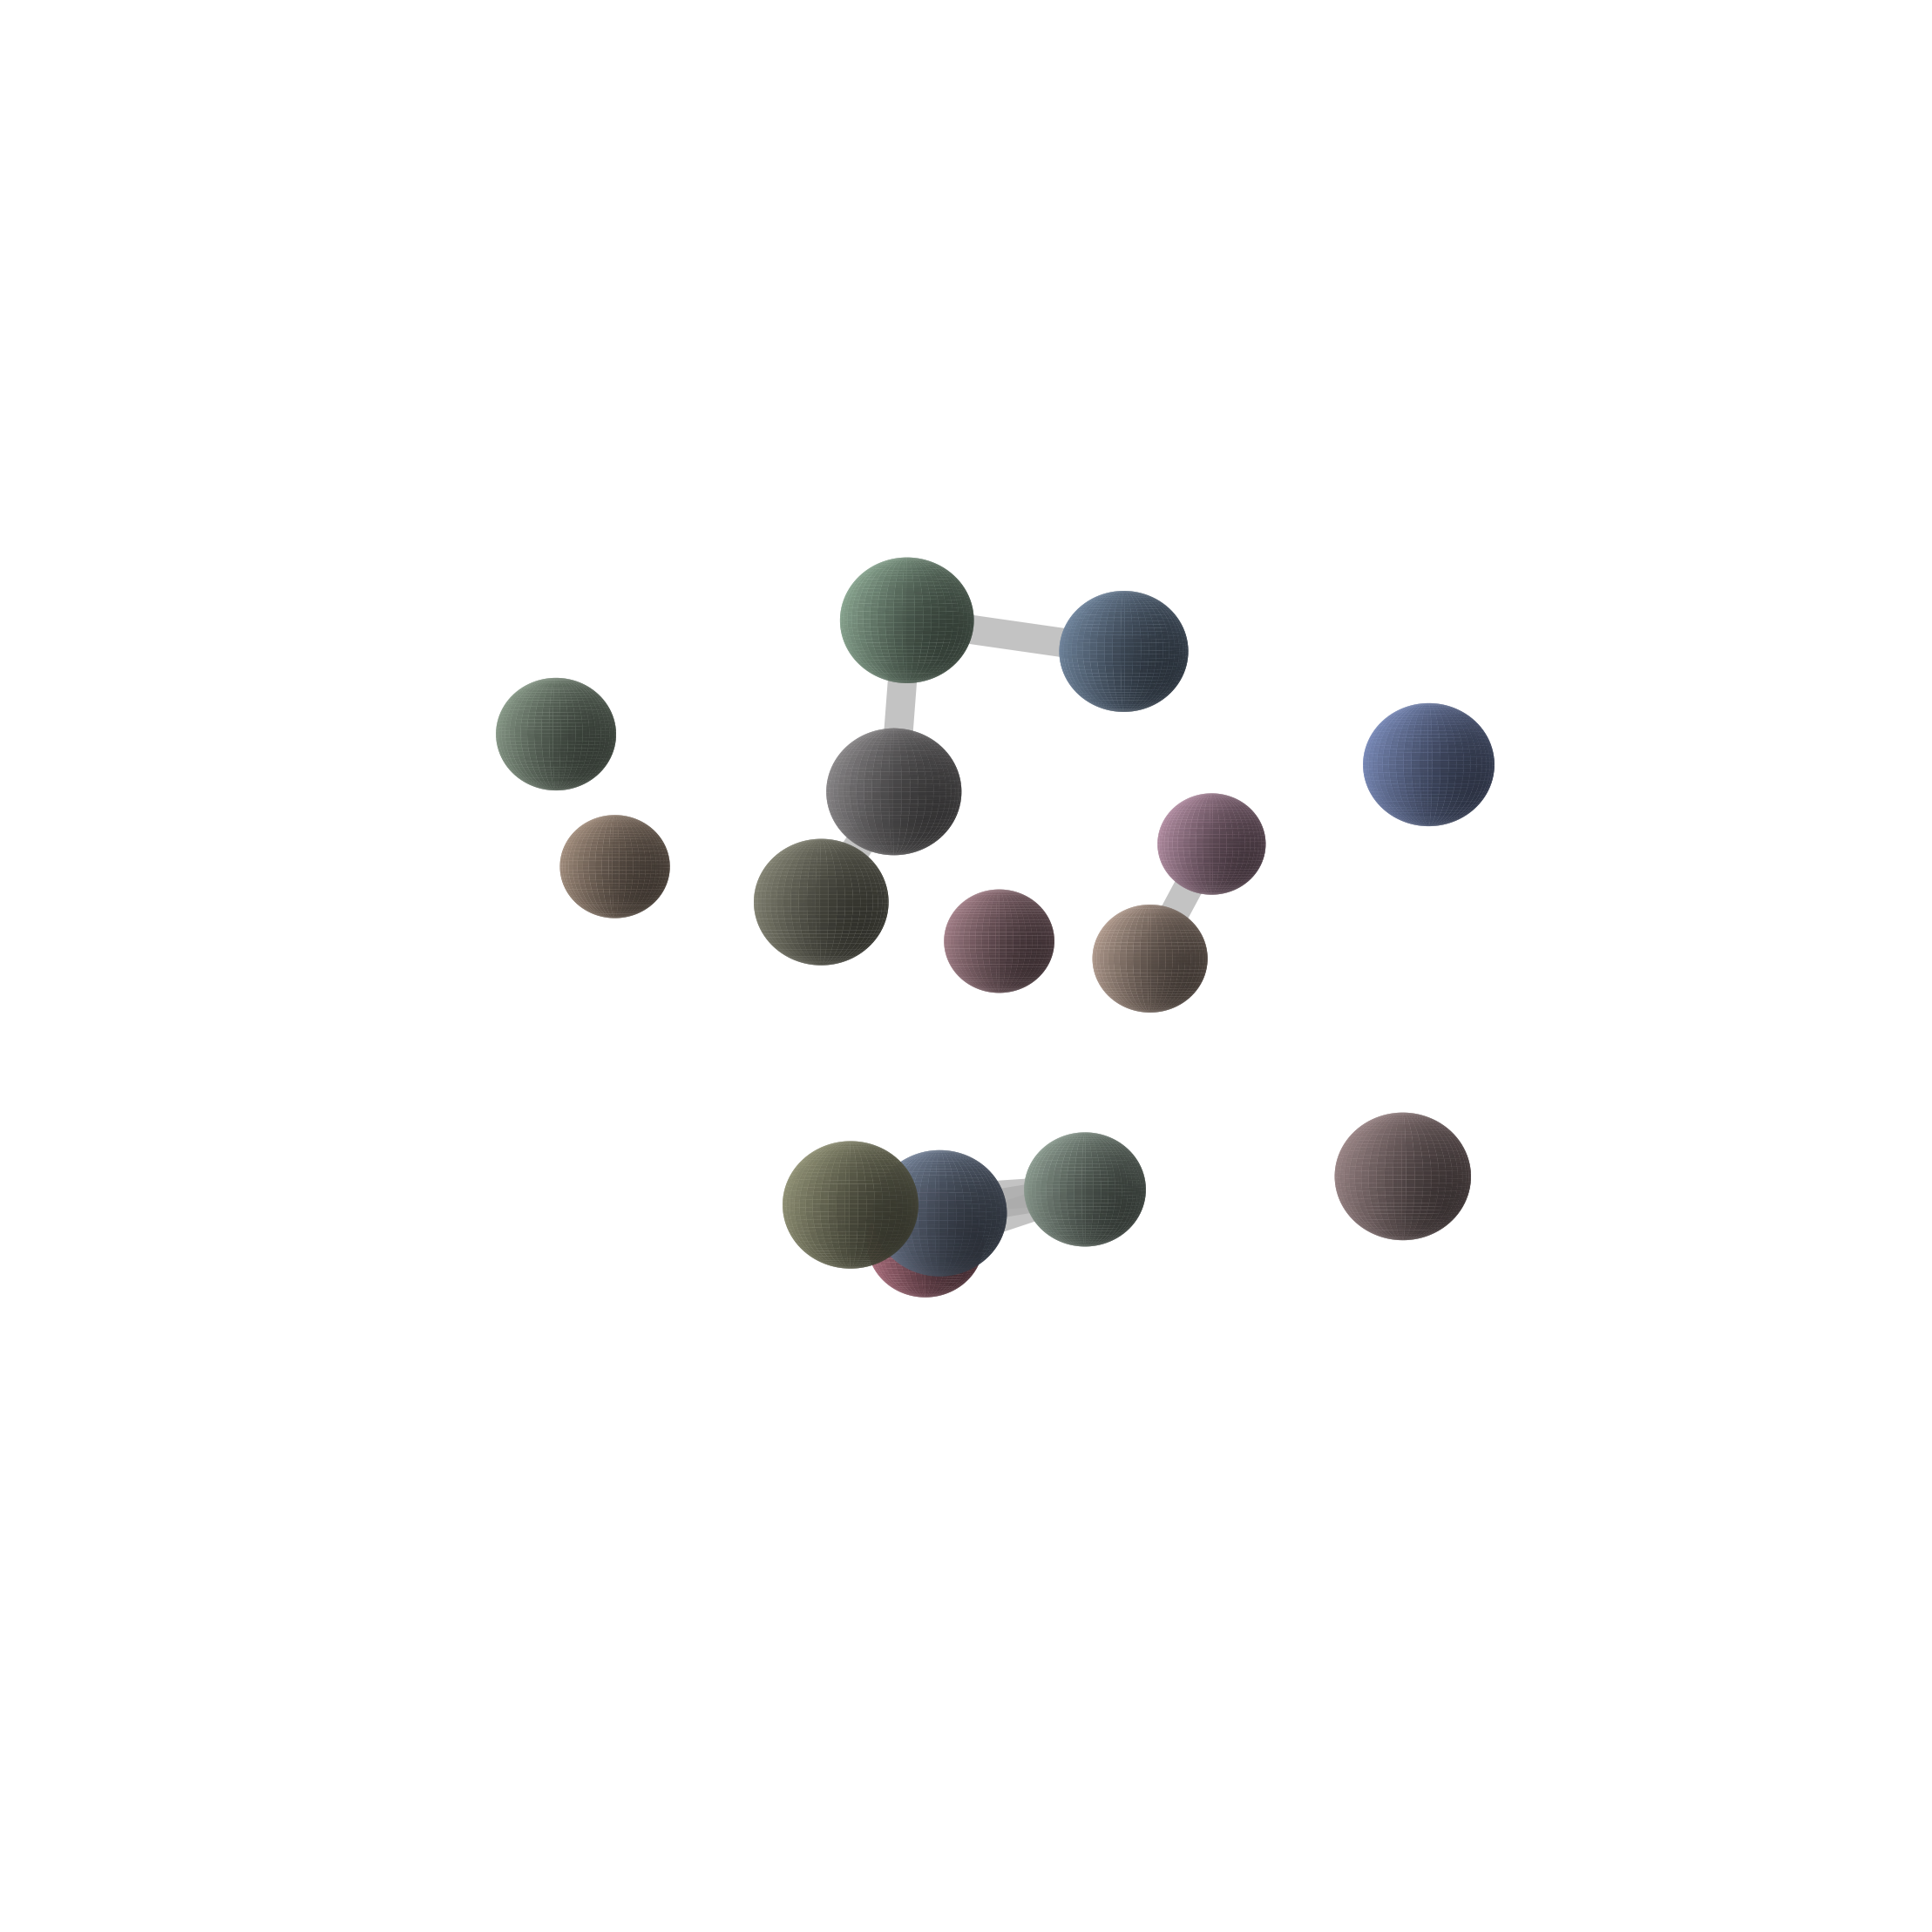
\includegraphics[width=\boxsize,height=\boxsize]{step_images/image_205.png}
  };
  \node[opacity=0.8] at (1.5*\boxsize + \gap, \boxsize/2 - 0.5em) {
    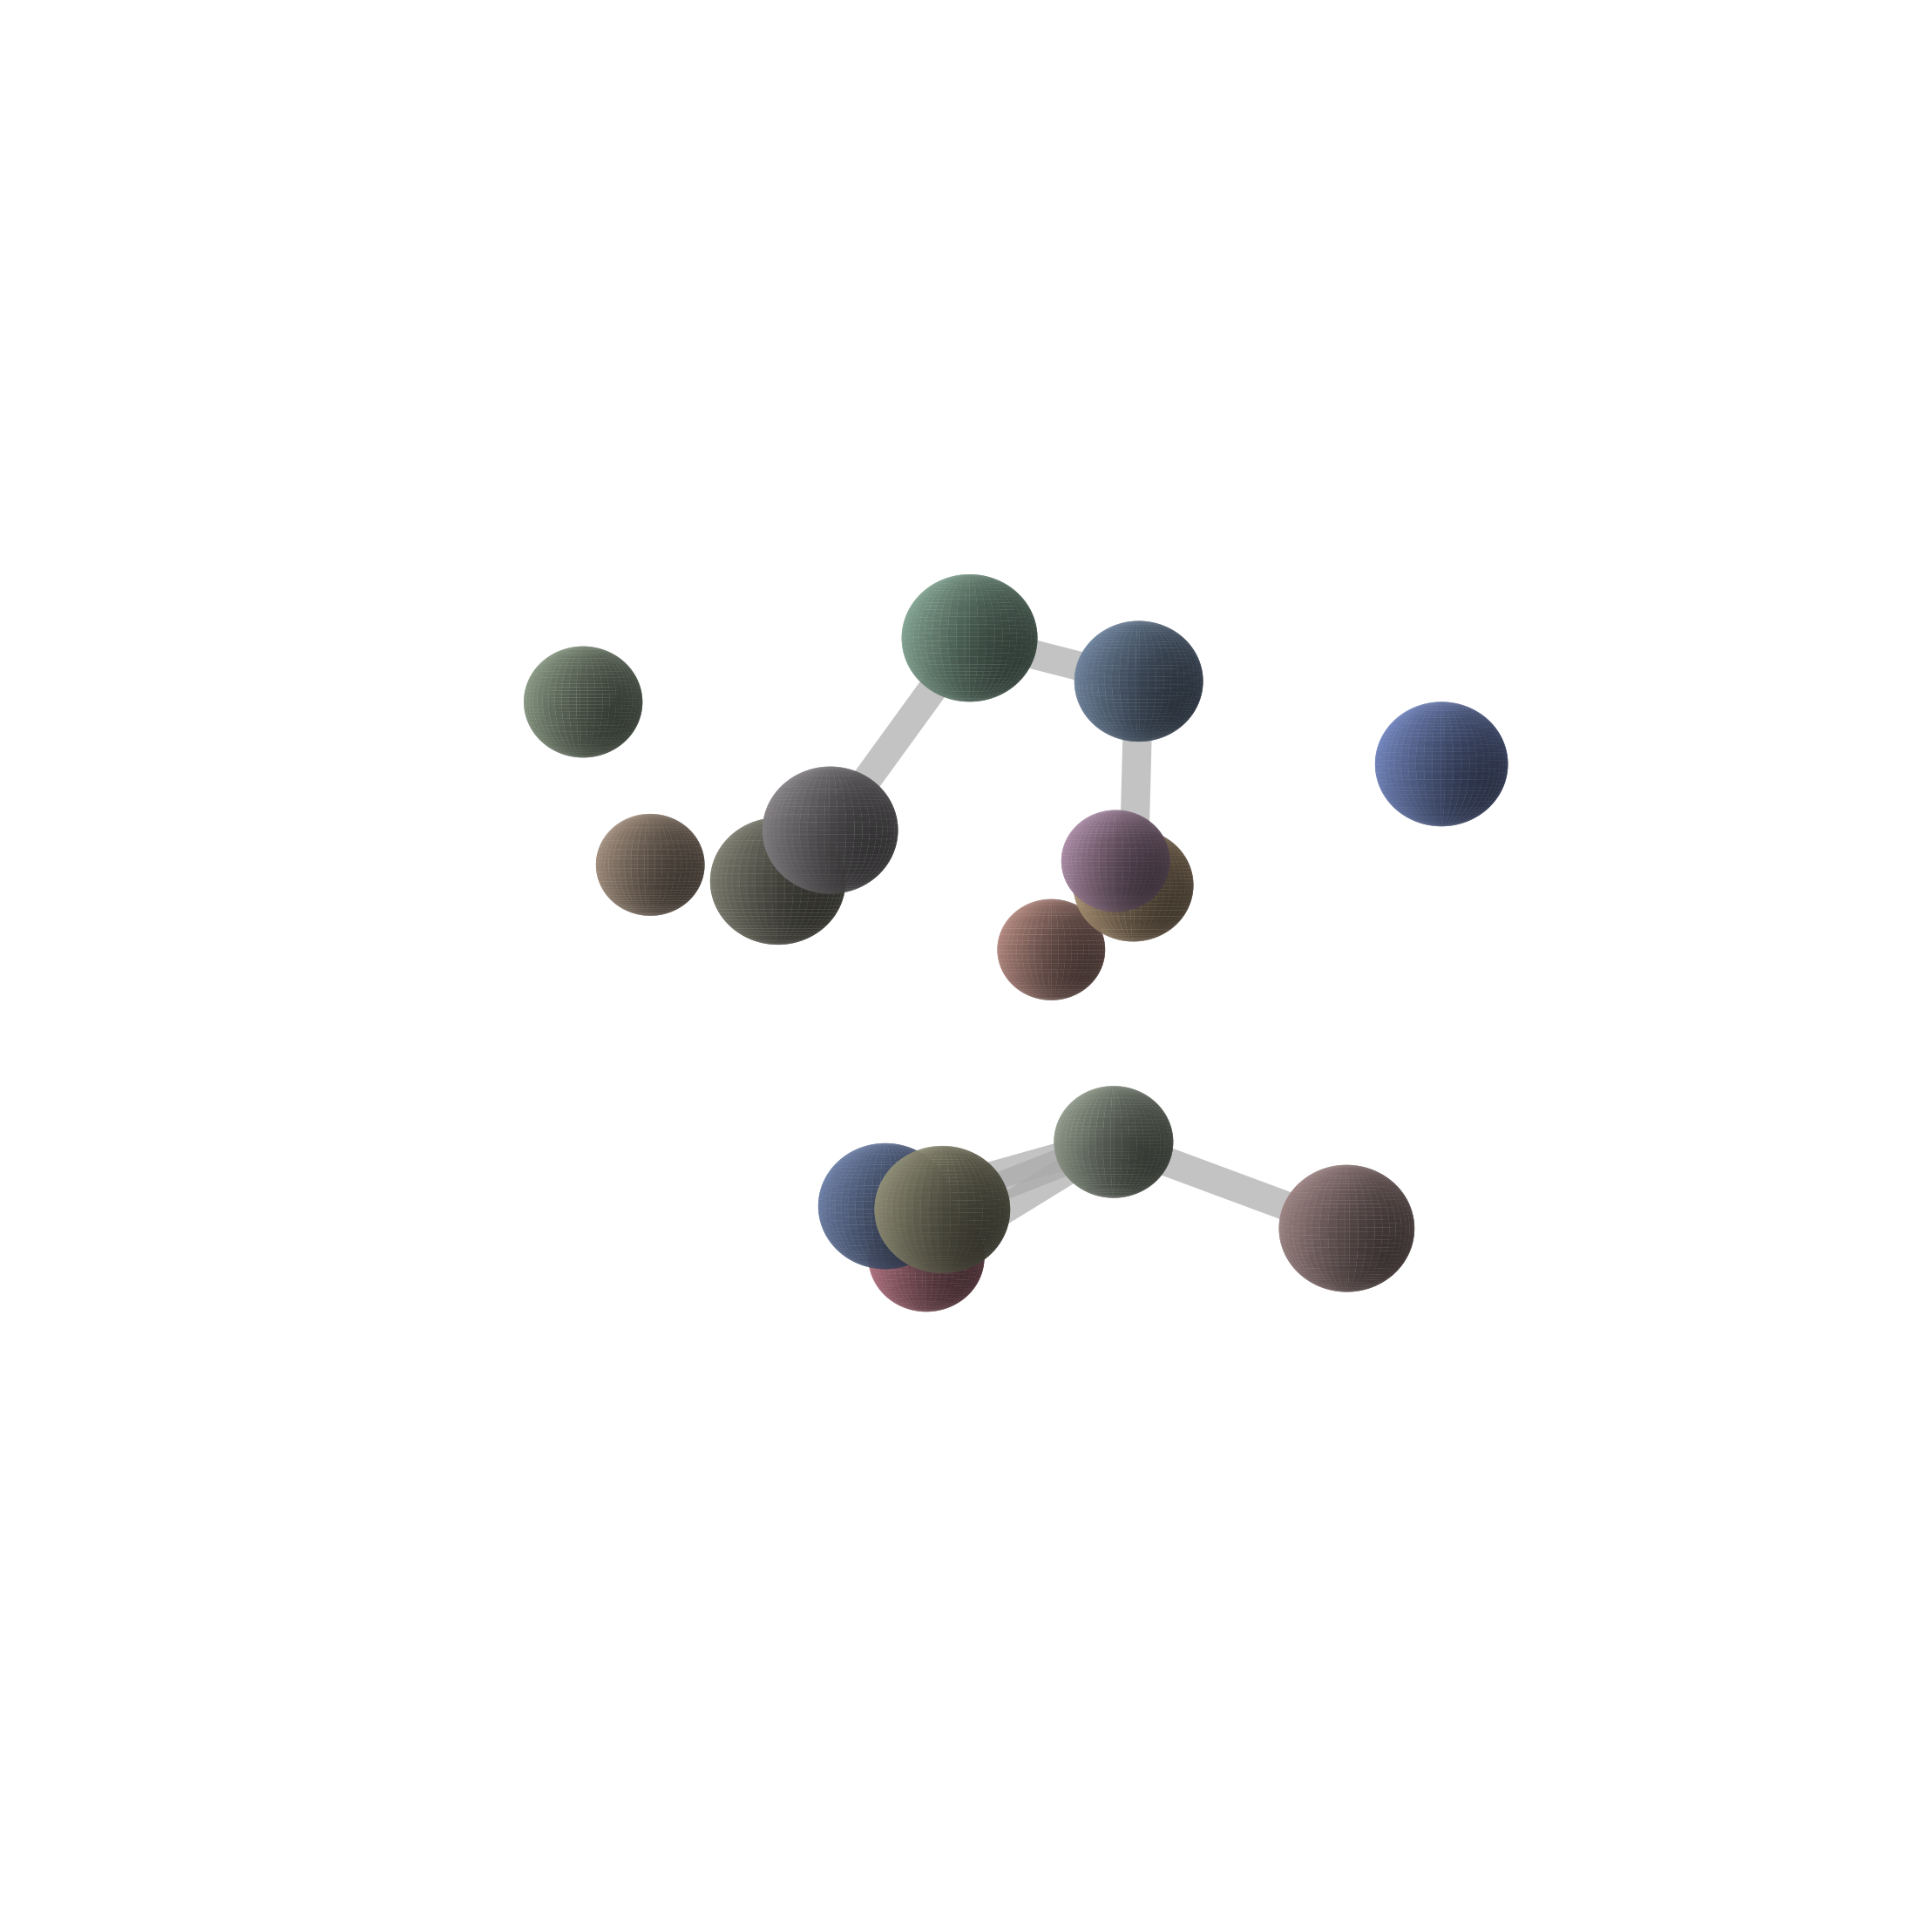
\includegraphics[width=\boxsize,height=\boxsize]{step_images/image_210.png}
  };

  \shade[bottom color=blue!20, top color=white] (2*\boxsize + 2*\gap,0) rectangle ++(\boxsize, \boxsize);
  \draw[thick] (2*\boxsize + 2*\gap,0) rectangle ++(\boxsize, \boxsize)node (C){};
  \node[opacity=0.8] at (2.5*\boxsize + 2*\gap, \boxsize/2 - 0.5em) {
    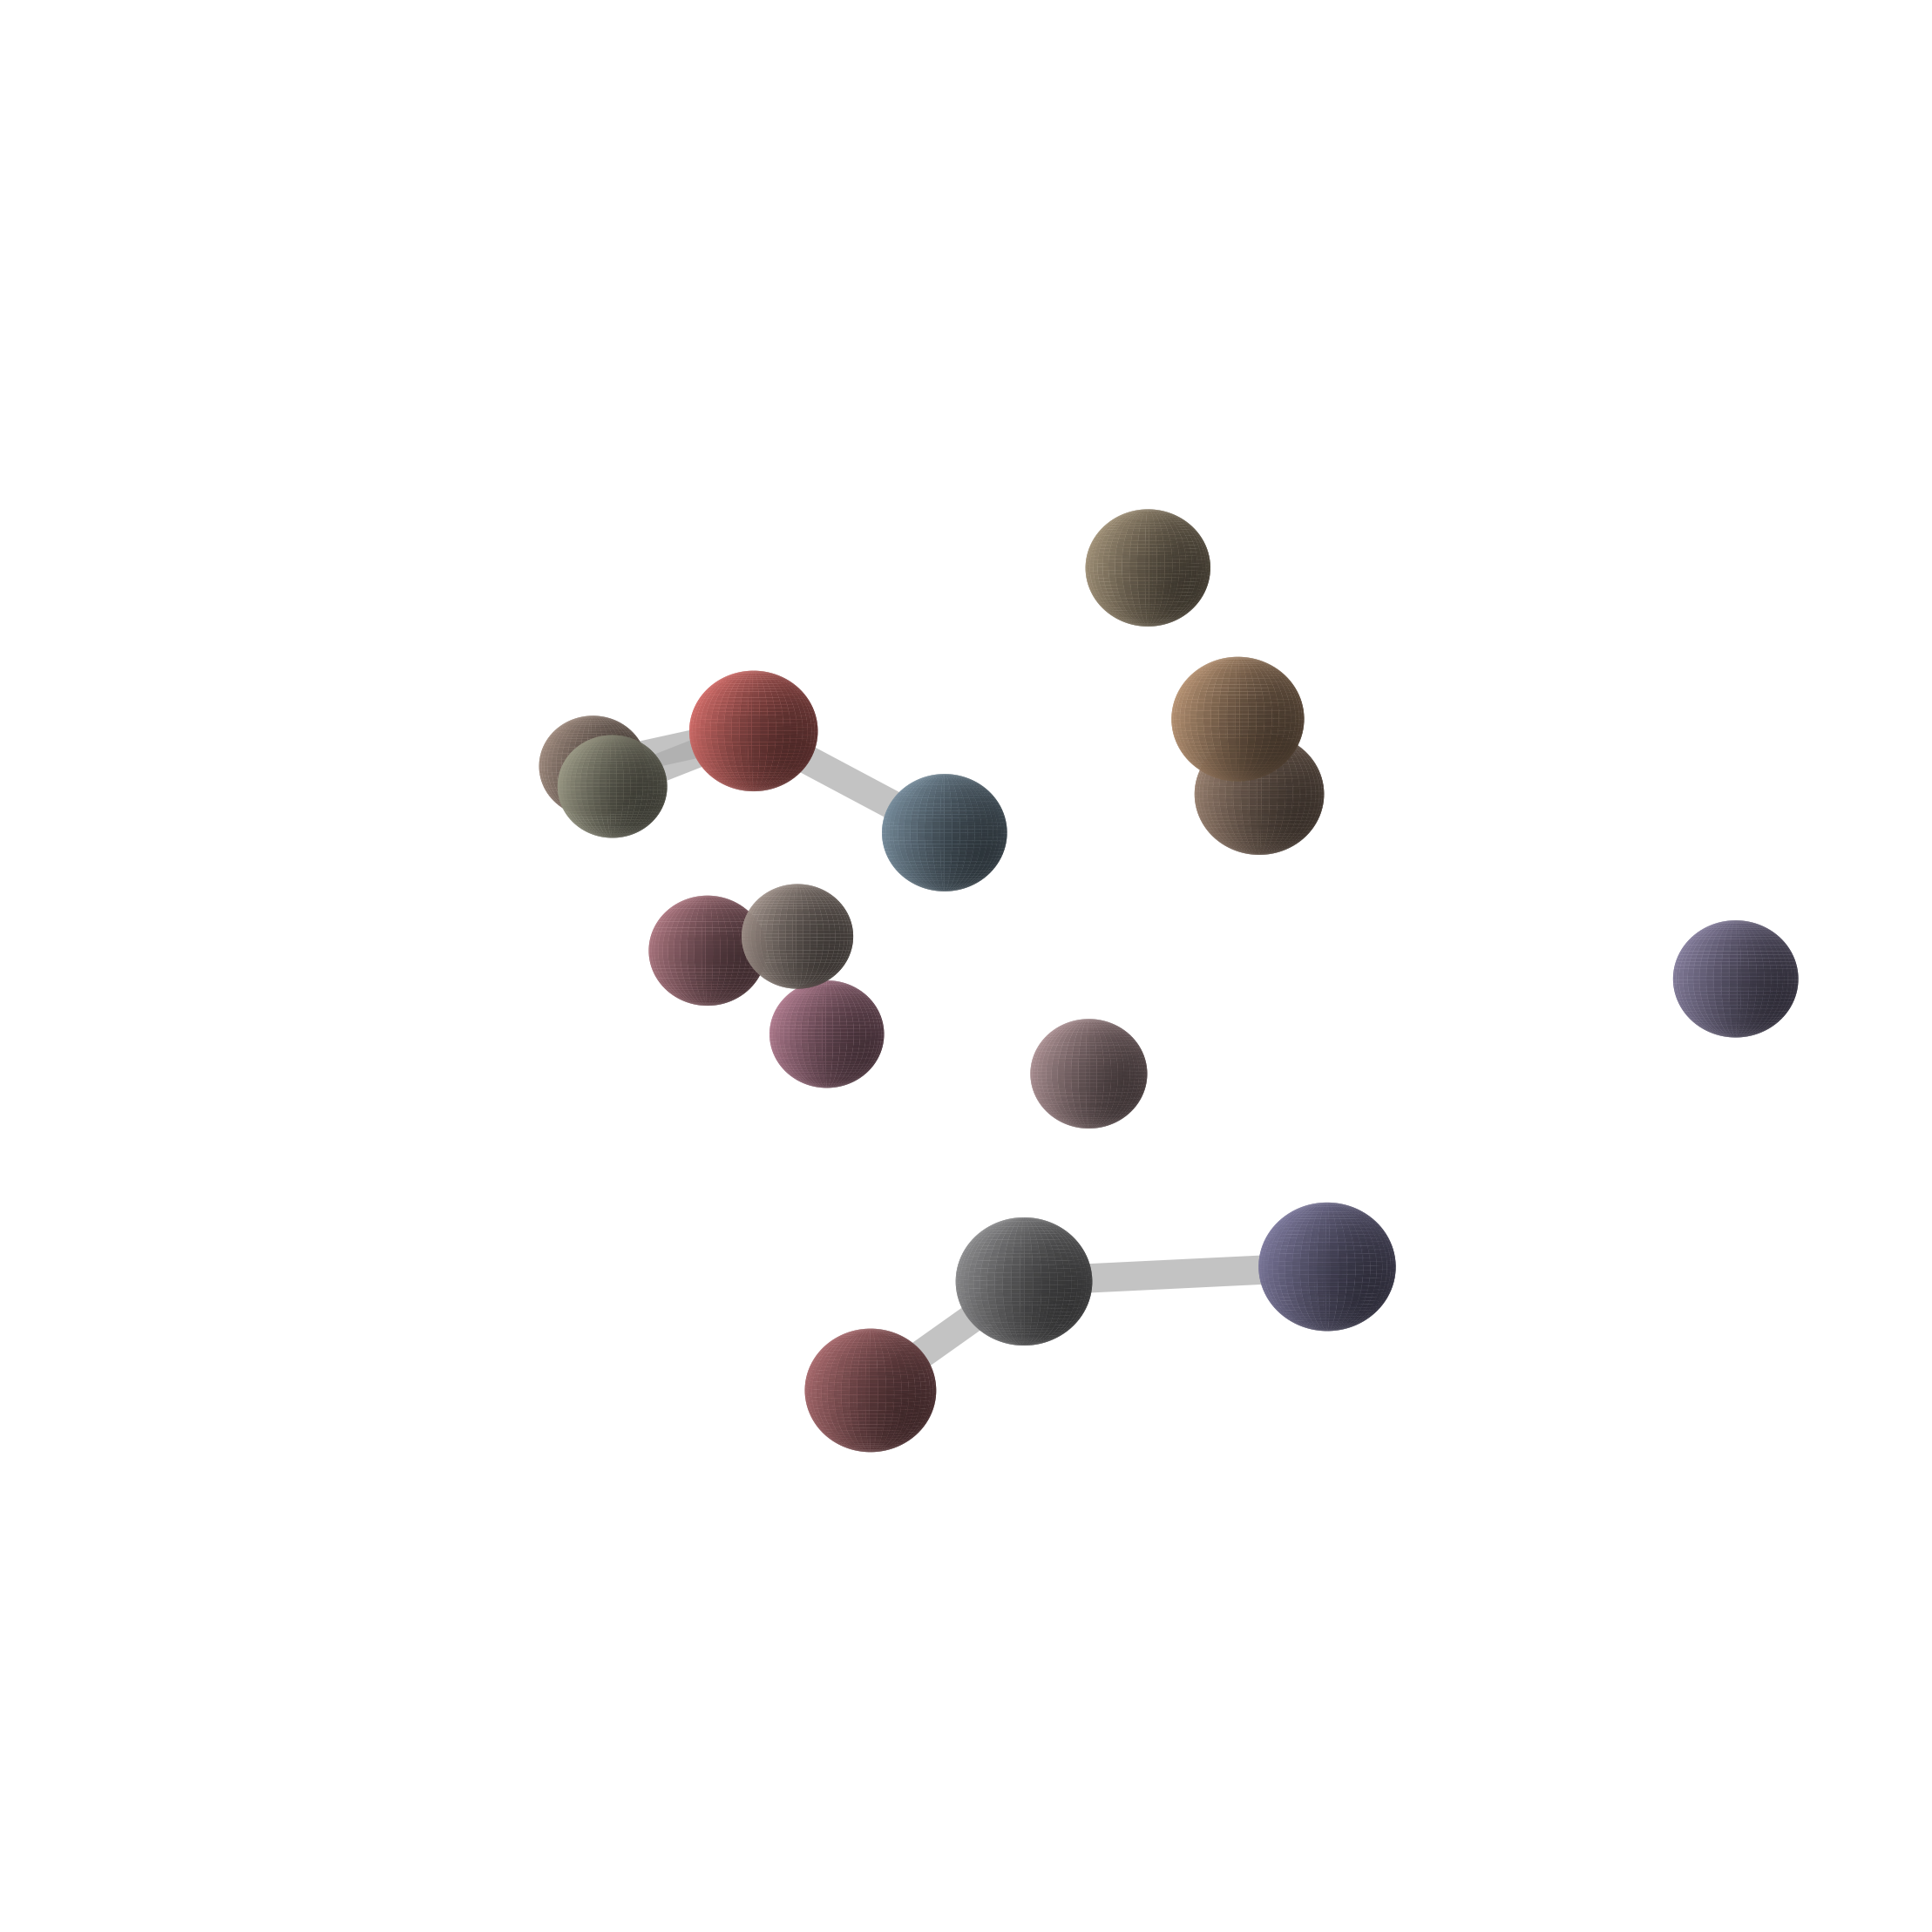
\includegraphics[width=\boxsize,height=\boxsize]{step_images/image_500.png}
  };
  \node[opacity=0.8] at (2.5*\boxsize + 2*\gap, \boxsize/2 - 0.5em) {
    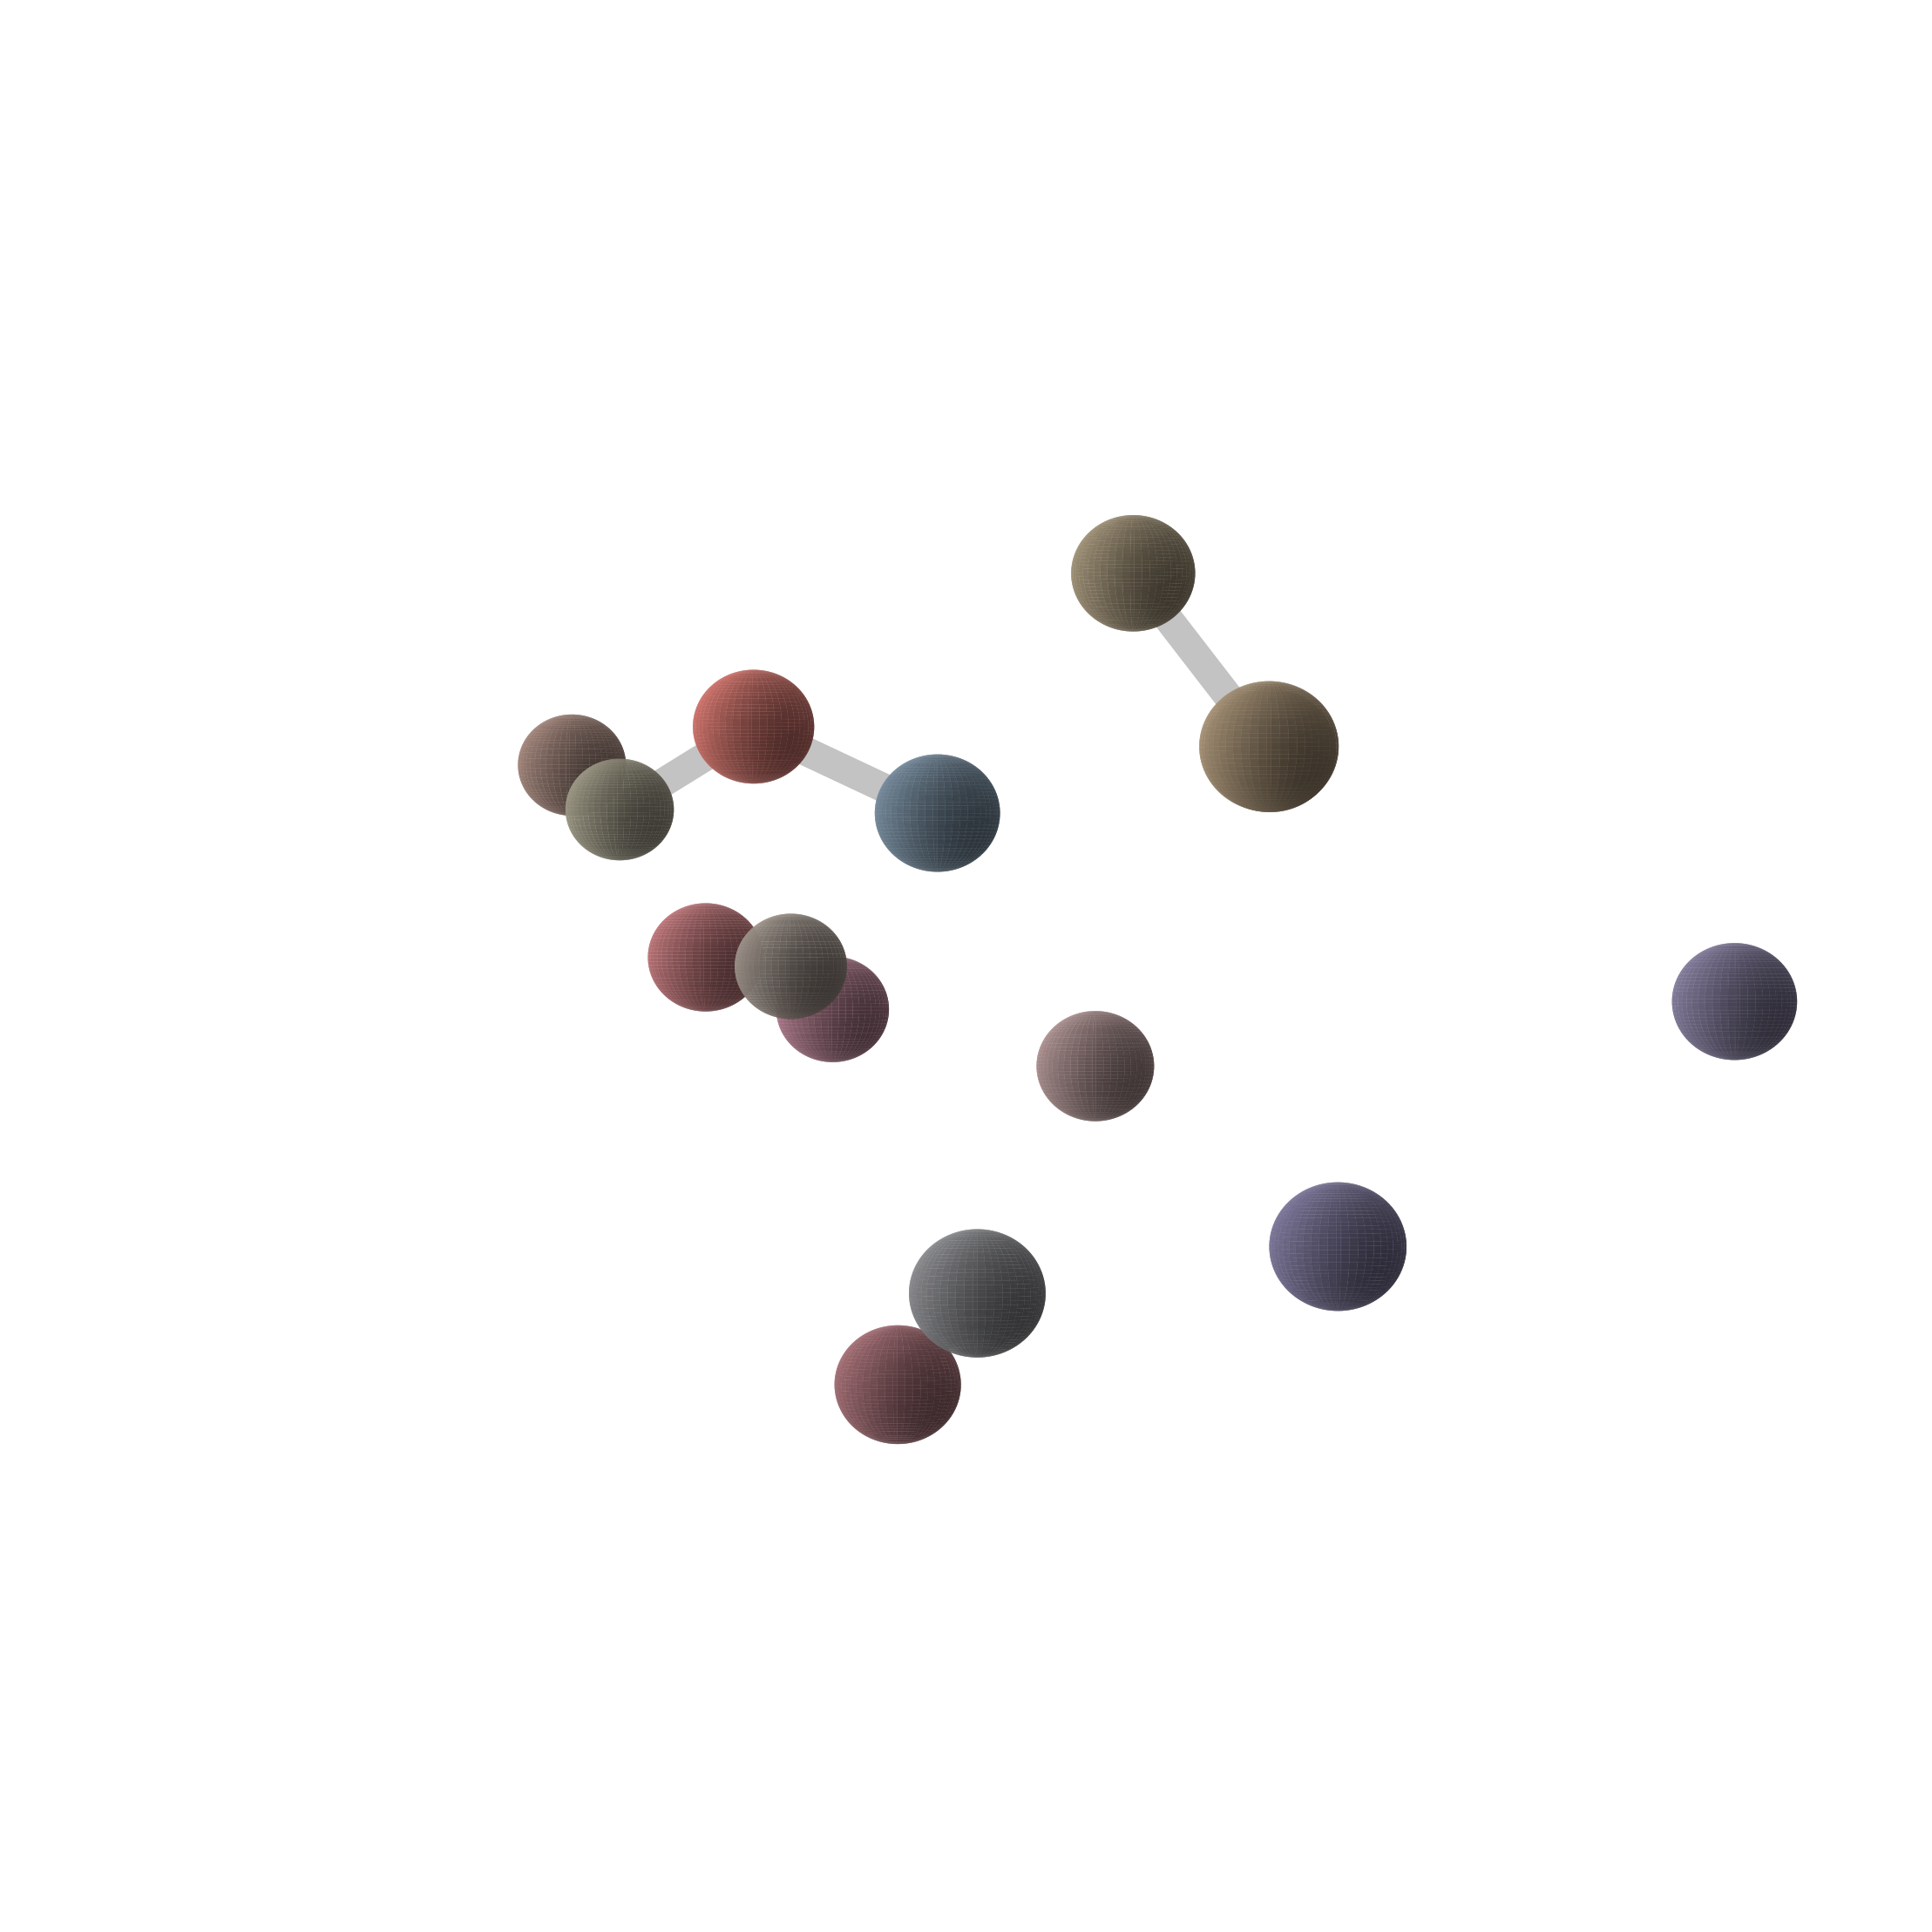
\includegraphics[width=\boxsize,height=\boxsize]{step_images/image_505.png}
  };
  \node[opacity=0.8] at (2.5*\boxsize + 2*\gap, \boxsize/2 - 0.5em) {
    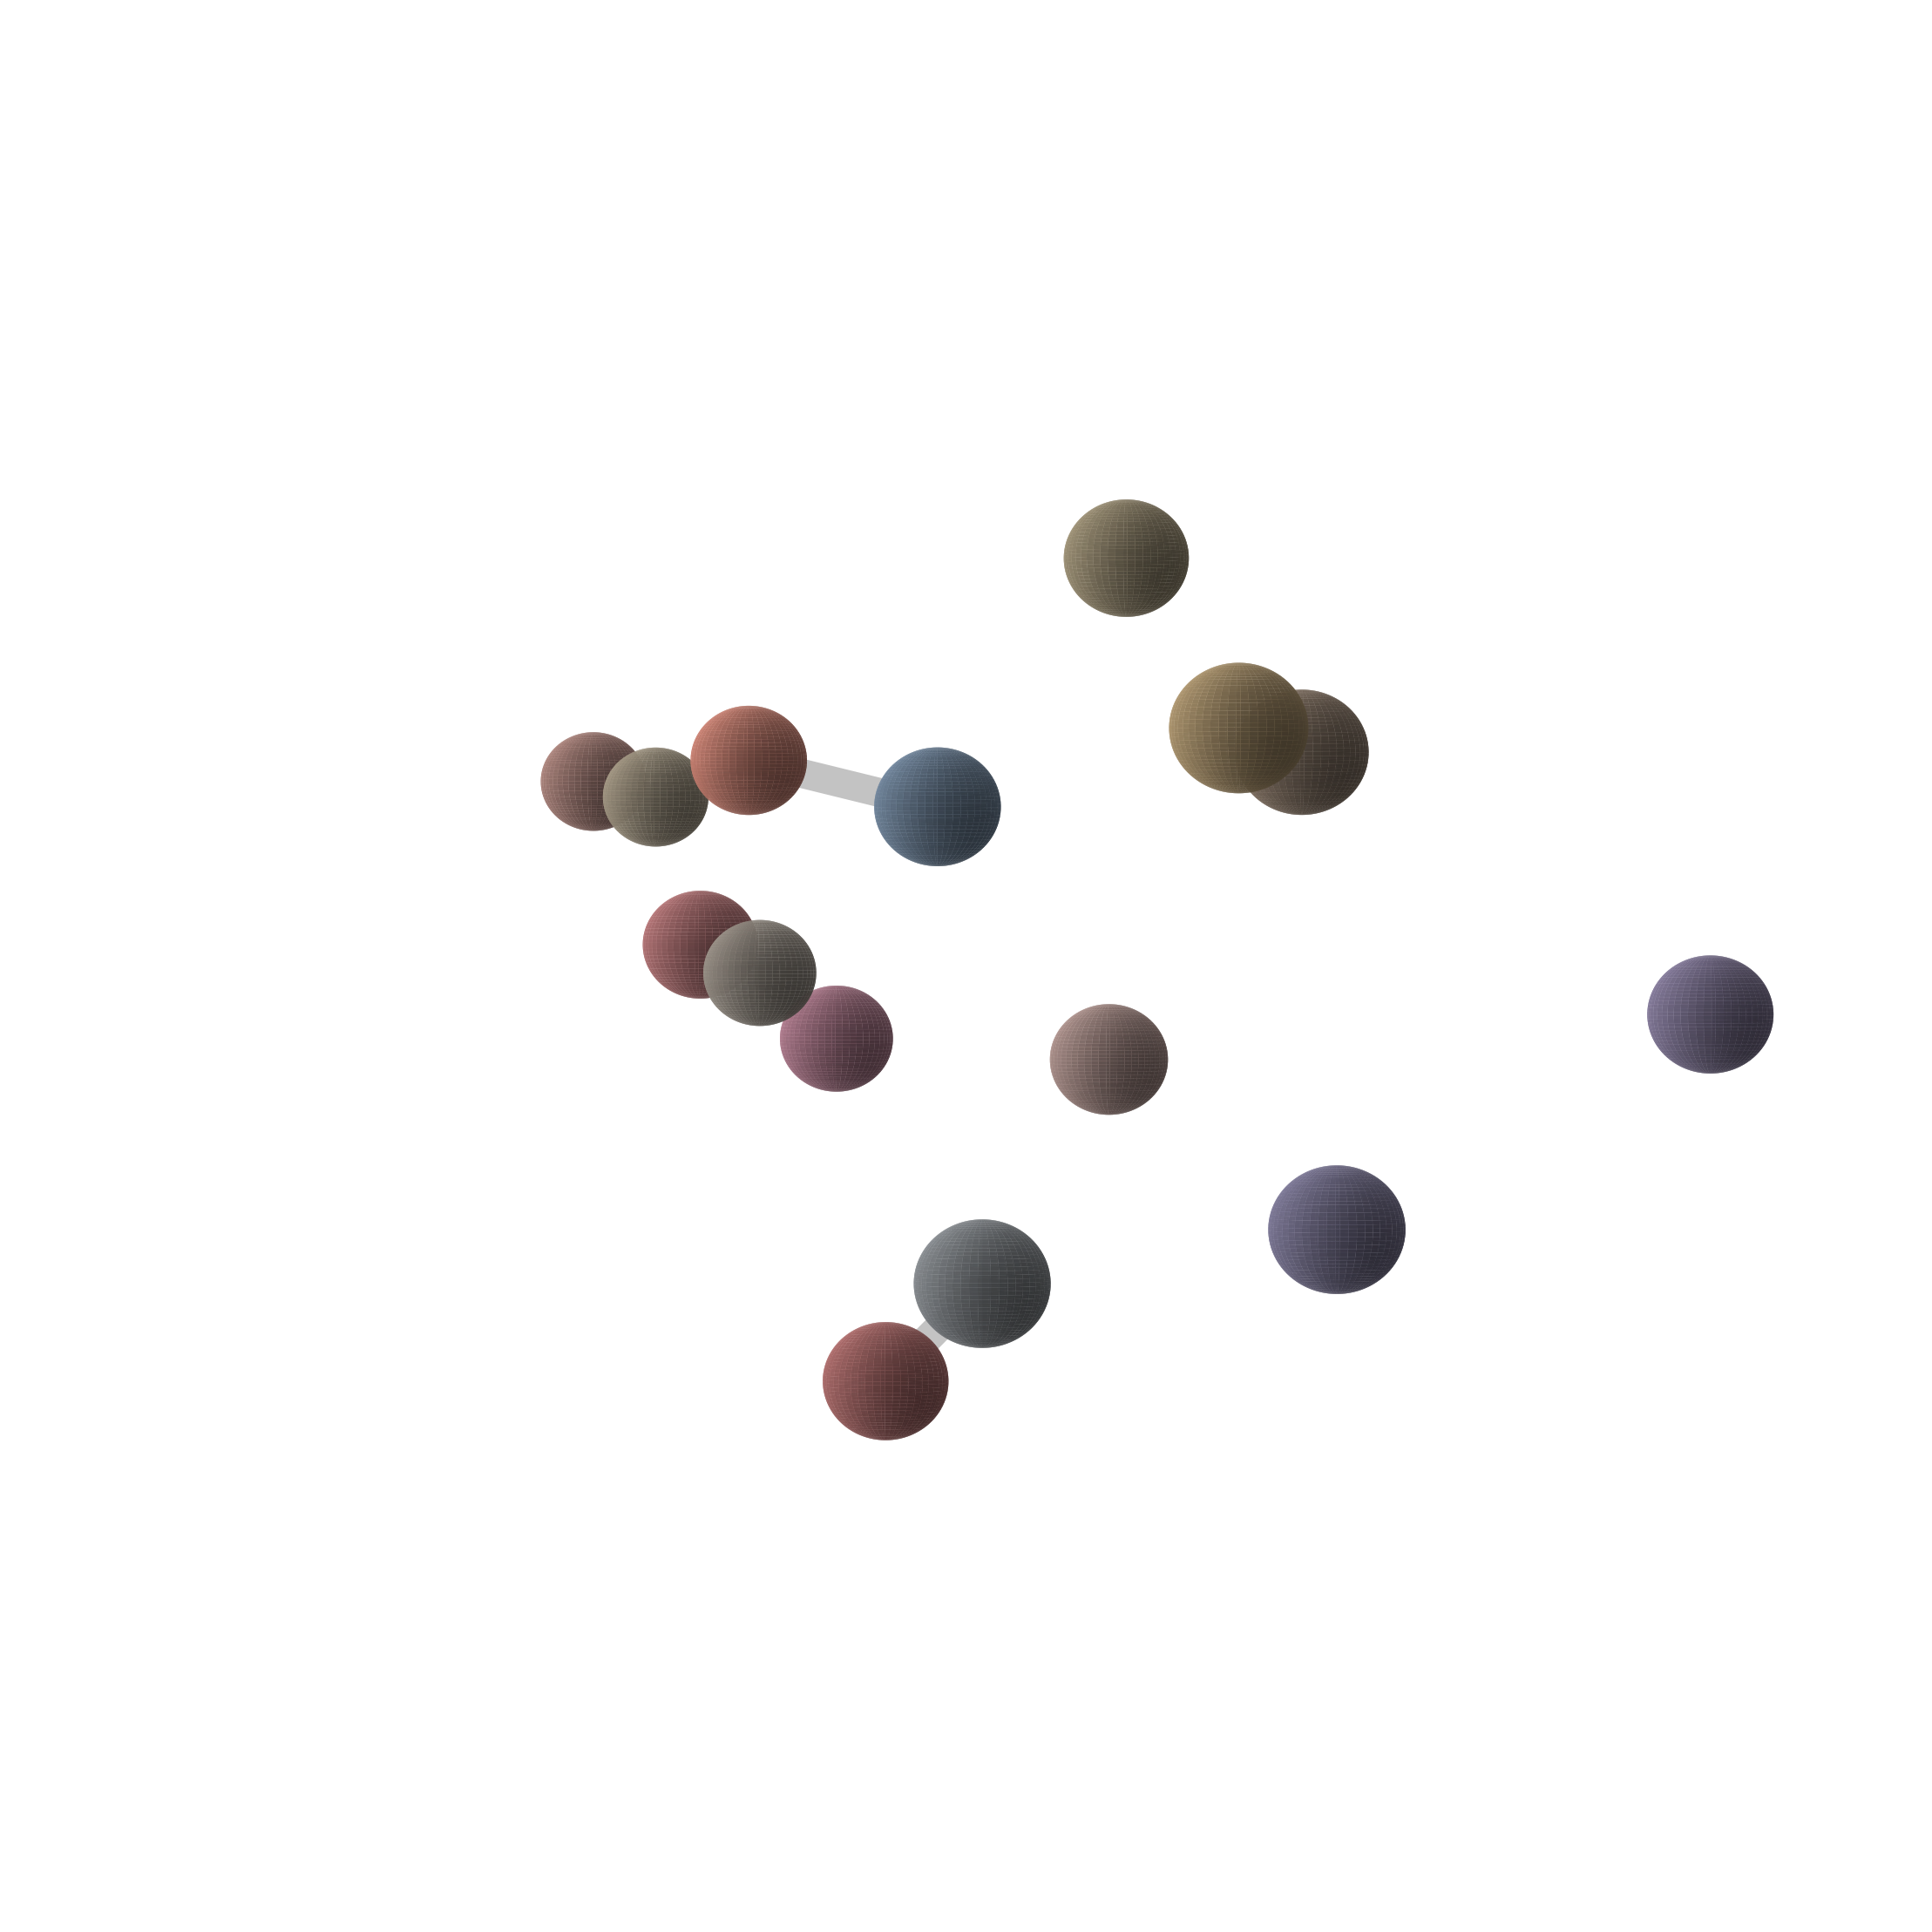
\includegraphics[width=\boxsize,height=\boxsize]{step_images/image_510.png}
  };

  \shade[bottom color=blue!20, top color=white] (3*\boxsize + 3*\gap + \gap,0) rectangle ++(\boxsize, \boxsize);
  \draw[thick] (3*\boxsize + 3*\gap + \gap,0) rectangle ++(\boxsize, \boxsize) node(D){};
  \node at (3.5*\boxsize + 3*\gap + \gap, \boxsize/2 - 0.5em) {
    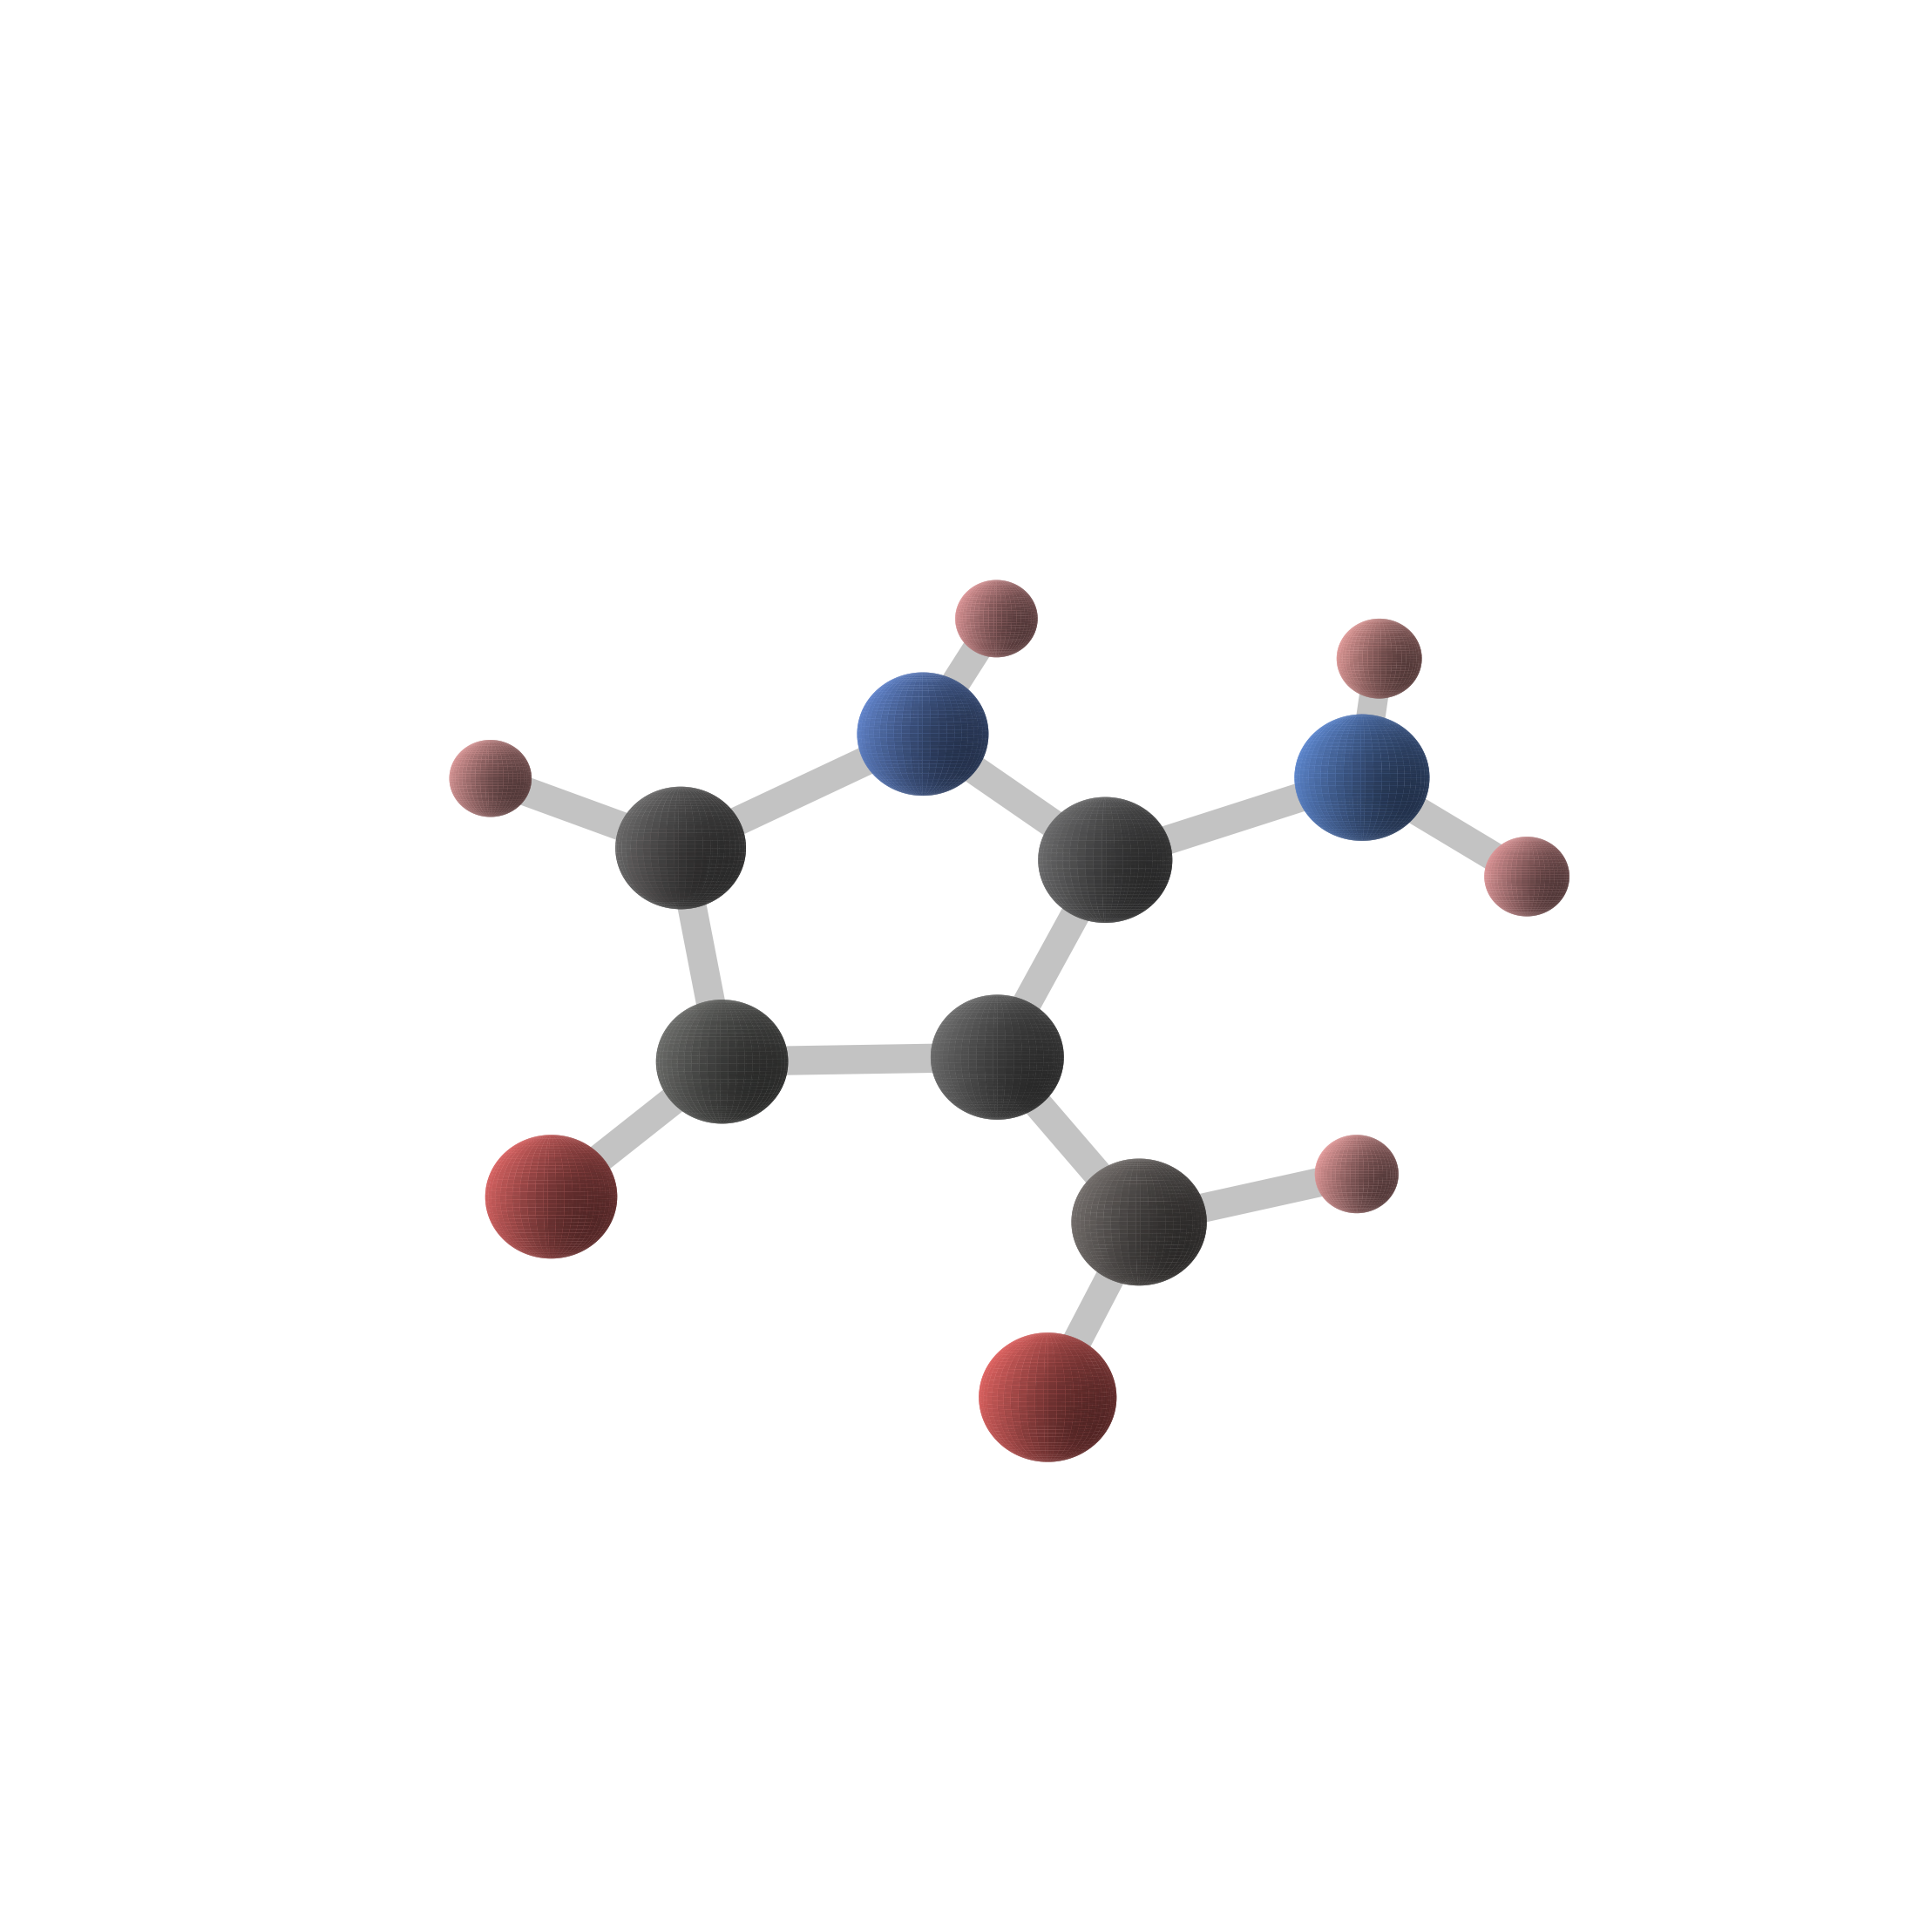
\includegraphics[width=\boxsize,height=\boxsize]{step_images/image_-2.png}
  };

  \shade[bottom color=blue!20, top color=white] (4*\boxsize + 4*\gap + \gap,0) rectangle ++(\boxsize, \boxsize);
  \draw[thick] (4*\boxsize + 4*\gap + \gap,0) rectangle ++(\boxsize, \boxsize) node (E){};
  \node at (4.5*\boxsize + 4*\gap + \gap, \boxsize/2 - 0.5em) {
    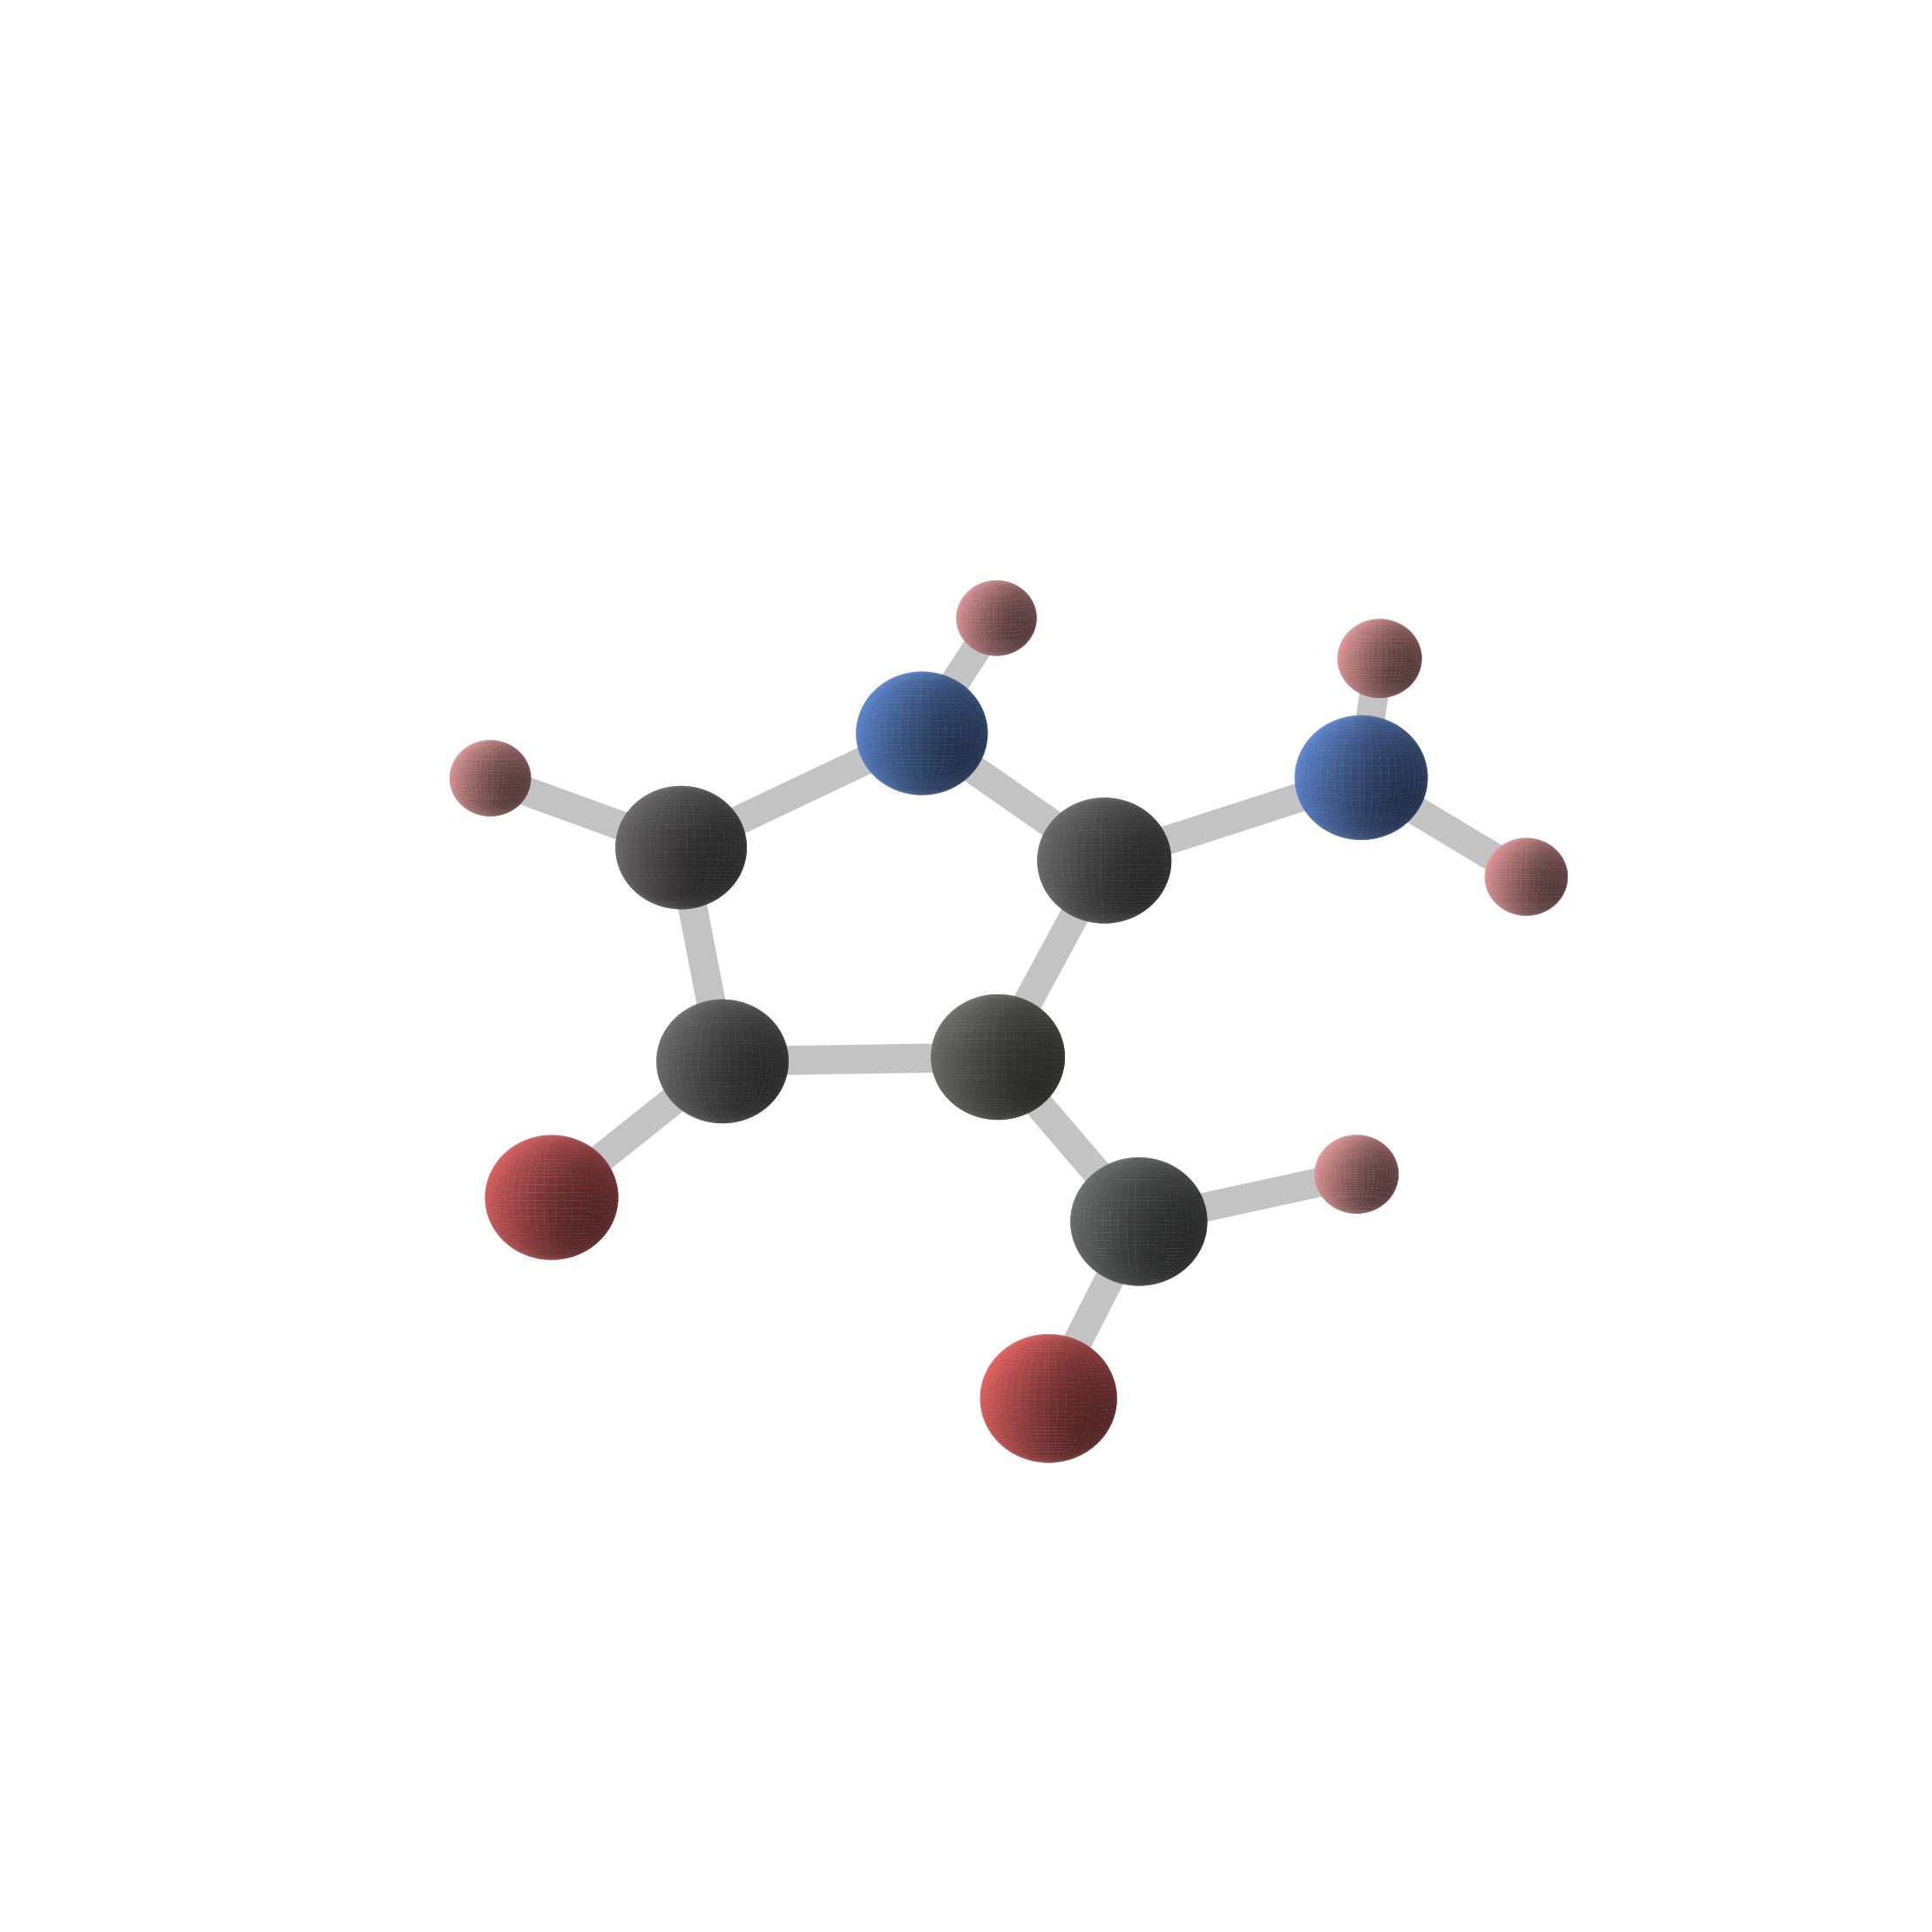
\includegraphics[width=\boxsize,height=\boxsize]{step_images/image_-1.png}
  };

  \draw[thick, -latex, dashed]($(A)-(\boxsize/2-2mm, -2mm)$) to [bend left,looseness=0.8] ($(B)-(\boxsize/2+2mm, -2mm)$);
  \draw[thick, -latex]($(B)-(\boxsize/2-2mm, -2mm)$) to [bend left,looseness=0.8] ($(C)-(\boxsize/2+2mm, -2mm)$);
  \draw[thick, -latex, dashed]($(C)-(\boxsize/2-2mm, -2mm)$) to [bend left,looseness=0.8] ($(D)-(\boxsize/2+2mm, -2mm)$);
  \draw[thick, -latex]($(D)-(\boxsize/2-2mm, -2mm)$) to [bend left,looseness=0.8] ($(E)-(\boxsize/2+2mm, -2mm)$);

  \draw[thick, latex-, dashed]($(B)-(\boxsize/2-2mm, \boxsize + 2mm)$) to [bend right,looseness=0.3] ($(E)-(\boxsize/2+2mm,  \boxsize+2mm)$);

  \node[above, align=center, baseline=0, inner sep=0, text height=2em, text depth=0] at (\boxsize/2-\gap, \boxsize + 8mm) {Pure noise: \\\(\operatorname{N}(\vb{0}, \mathbf{I})\)};

  \node[above, align=center, baseline=0, inner sep=0, text height=2em, text depth=0] at (1.5*\boxsize + 1.5*\gap + \boxsize/2, \boxsize + 8mm) {Denoise: \\\(p_{\theta}(\vb{z}_{t-1} \mid \vb{z}_{t})\)};

  \node[above, align=center, baseline=0, inner sep=0, text height=2em, text depth=0] at (4*\boxsize + 3*\gap + \boxsize/2, \boxsize + 8mm) {Decode: \\\(p_{\theta}(\vb{x} \mid \vb{z}_{0})\)};

  \node[below, align=center, baseline=0, inner sep=0, text height=2em, text depth=0] at (3*\boxsize + 3*\gap, - 8mm) {Add noise: \\\(q(\vb{z}_{t} \mid \vb{x})\)};

  \node[below, align=center, baseline=0, inner sep=0, text height=1.5em, text depth=0] at (0.5*\boxsize-\gap, \boxsize) {\(\vb{z}_{T}\)};
  \node[below, align=center, baseline=0, inner sep=0, text height=1.5em, text depth=0] at (1.5*\boxsize + 1*\gap, \boxsize) {\(\vb{z}_{t}\)};
  \node[below, align=center, baseline=0, inner sep=0, text height=1.5em, text depth=0] at (2.5*\boxsize + 2*\gap, \boxsize) {\(\vb{z}_{t-1}\)};
  \node[below, align=center, baseline=0, inner sep=0, text height=1.5em, text depth=0] at (3.5*\boxsize + 3*\gap + \gap, \boxsize) {\(\vb{z}_{0}\)};
  \node[below, align=center, baseline=0, inner sep=0, text height=1.5em, text depth=0] at (4.5*\boxsize + 4*\gap + \gap, \boxsize) {\(\vb{x}\)};

  \node at (\boxsize, 0.5 * \boxsize) {\textbf{...}};
  \node at (3*\boxsize + 3*\gap, 0.5 * \boxsize) {\textbf{...}};

\end{tikzpicture}

\end{document}
